% SETTINGS - LATEX
% to change name, title, supervisor etc. go to preamble/preamble.tex
\newcommand{\myFontSize}[0] {12pt}
\newcommand{\mySpacing}[0] {1.5}
\newcommand{\myBibliography}[0] {bib/refs, appendices/refs1}

\documentclass[12pt,a4paper,twoside]{book}

% Use babel for language support
\usepackage[english]{babel}

\usepackage[utf8]{inputenc}
\usepackage[T1]{fontenc}
\usepackage[a4paper]{geometry}
\usepackage[
    left = \glqq,% 
    right = \grqq,% 
    leftsub = \glq,% 
    rightsub = \grq%
]{dirtytalk}

% SETTINGS - NAMES
\newcommand{\myTitle}[0] {Histological Image Data Processing Using Methods of Computer Vision and Deep Neural Networks}
\newcommand{\myName}[0] {Martin Sivák}
\newcommand{\mySupervisor}[0] {prof. Ing. Vanda Benešová, PhD.}
\newcommand{\myEvidenceNumber}[0] {FIIT-XXXX-XXXXX}
\newcommand{\myDate}[0] {May 2025}
\newcommand{\myStudyProgram}[0] {Informatics}
\newcommand{\myDegreeCourse}[0] {Computer Science}
\newcommand{\myInstitute}[0] {Institute of Informatics and Software Engineering, FIIT STU, Bratislava}

\usepackage[parfill]{parskip}
\usepackage{enumitem}

\usepackage{graphicx}
\usepackage{float}
\usepackage{longtable}
\usepackage{setspace}
\usepackage{amsmath} % for math formatting
\usepackage{amssymb} % for math formatting
\usepackage{multicol} % for side-by-side equations

% Spacing
\setstretch{\mySpacing}

\setcounter{secnumdepth}{3}
\setcounter{tocdepth}{3}

\usepackage{tabularx}
\newsavebox\mybox
\usepackage{fancyhdr}
\pagestyle{fancy}
\lhead{\nouppercase{\leftmark}}
\chead{}
\rhead{}
\lfoot{}
\cfoot{\thepage}
\rfoot{}


%style=iso-numeric
%style=authortitle-dw
\usepackage[backend=biber,sorting=none, defernumbers=true, style=numeric]{biblatex}
\defbibheading{references}[References]{ 
  \chapter*{#1}
  \markboth{#1}{#1}
}
\defbibheading{referencessec}[References]{ 
  \section*{#1}
  \markboth{#1}{#1}
}
\bibliography{\myBibliography}


% Listing as figure
%\usepackage{libs/minted}
%\usepackage[section]{minted}

\usepackage{listing}

% openright does not work :(
\let\tmp\oddsidemargin
\let\oddsidemargin\evensidemargin
\let\evensidemargin\tmp
\reversemarginpar

\usepackage{lscape}
\usepackage{afterpage}

\usepackage{lipsum}

\begin{document}

\raggedbottom % to prevent extensive stretching of content

% Minted
% pygmentize -L styles
%\usemintedstyle{autumn}

% Title page

\begin{center}
\thispagestyle{empty}
{\Large Slovenská technická univerzita v Bratislave}
\par\end{center}{\Large \par}

\begin{center}
{\Large Fakulta informatiky a informačných technológií}
\par\end{center}{\Large \par}

\smallskip{}

\begin{center}
\myEvidenceNumber
\par\end{center}
\vfill{}

\begin{center}
\textbf{\Large \myName}
\par\end{center}{\Large \par}

\medskip{}


\begin{center}
\textbf{\LARGE \myTitle }
\par\end{center}{\huge \par}

\medskip{}


\begin{center}

{\Large Priebežná správa o riešení BP1}
\par\end{center}{\Large \par}

\vfill{}

Supervisor: \mySupervisor

\medskip{}
\myDate

\pagenumbering{roman}

\newpage
\thispagestyle{empty}
\mbox{}
\newpage



\begin{center}
\thispagestyle{empty}
{\Large Slovenská technická univerzita v Bratislave}
\par\end{center}{\Large \par}

\begin{center}
{\Large Fakulta informatiky a informačných technológií}
\par\end{center}{\Large \par}

\smallskip{}

\begin{center}
\myEvidenceNumber
\par\end{center}
\vfill{}

\begin{center}
\textbf{\Large \myName}
\par\end{center}{\Large \par}

\medskip{}


\begin{center}
\textbf{\LARGE \myTitle }
\par\end{center}{\huge \par}

\medskip{}


\begin{center}

{\Large Priebežná správa o riešení BP1}
\par\end{center}{\Large \par}

\vfill{}

Study program: \myStudyProgram

Degree course: \myDegreeCourse

Place of elaboration: \myInstitute

Supervisor: \mySupervisor

\medskip{}

\myDate


\newpage
\thispagestyle{empty}
\mbox{}
\newpage

\newgeometry{top=0in, bottom=0in, left=0in, right=0in} % Set zero margin for this page
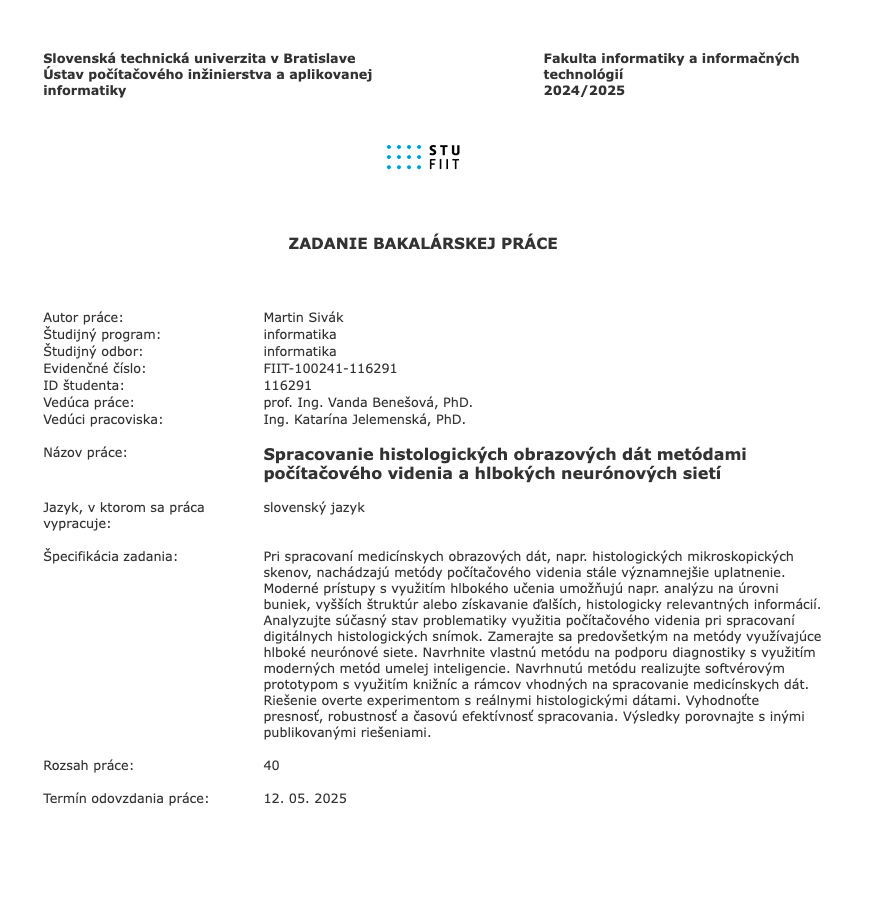
\includegraphics[width=\paperwidth]{assets/images/task-desc.png}
\restoregeometry % Revert to original margins
\newpage
\thispagestyle{empty}
\mbox{}
\newpage



% Annotation

\thispagestyle{empty}

\section*{Annotation}

\begin{minipage}[t]{1\columnwidth}%
Slovak University of Technology, Bratislava 

Faculty of Informatics and Information Technologies

Degree Course: \myStudyProgram\\

Author: \myName

Bachelor's Thesis: \myTitle

Supervisor: \mySupervisor

\myDate%
\end{minipage}

\bigskip{}

%Breast cancer is one of the leading causes of death among women, and accurate histopathological analysis plays a significant role in diagnosis and treatment planning. Tumor-infiltrating lymphocytes (TILs) have emerged as a promising biomarker. However, manual analysis and counting of TILs in histopathological slides remain time-consuming, error-prone, and require skilled professionals. Deep learning models have shown promise in automating this process, but they depend on large amounts of high-quality annotated data. 

In this thesis, we look at state-of-the-art weak segmentation techniques in digital pathology, focusing on segmenting lymphocyte cell nuclei in breast cancer patients. The main challenge stems from the weak annotations of nuclei in the form of bounding boxes instead of exact pixel-level masks. To tackle this challenge, we introduce a hybrid approach, where we use traditional computer vision techniques, such as Otsu and adaptive thresholding, and marked watershed, to create pixel-level pseudo-masks that are used to train a U-Net model. 
We show that using a small, although fully annotated, dataset is insufficient to train the model. Next, we try training the model on the pseudo-masks created by different computer vision pipelines, on the large weakly annotated dataset. To use the combined strength of different pseudo-masks, we then try creating a second generation of them by trying various fusion strategies. Finally, we try a transfer learning approach, where a model pretrained on a large dataset with pseudo-masks is fine-tuned on a small, fully annotated dataset. We evaluate each model on quantitative metrics such as Dice coefficient and Intersection over Union, and qualitative metrics by visualizing its predictions.

% english annotation content here


\newpage{}\thispagestyle{empty}



\thispagestyle{empty}
\section*{Anotácia}

\begin{minipage}[t]{1\columnwidth}%
Slovenská technická univerzita v Bratislave

Fakulta informatiky a informačných technológií

Študijný program: Informatika\\

Autor: \myName

Bakalárska práca: \myTitle

Vedúci bakalárskeho projektu: \mySupervisor

\myDateSK%
\end{minipage}

\bigskip{}

V tejto práci sa zaoberáme technikami slabej segmentácie v digitálnej patológii so zameraním na segmentáciu jadier buniek lymfocytov u pacientov s rakovinou prsníka. Hlavná výzva vyplýva zo slabých anotácií jadier vo forme ohraničujúcich rámčekov namiesto presných masiek na úrovni pixelov. Na riešenie tejto výzvy zavádzame hybridný prístup, v ktorom používame tradičné techniky počítačového videnia, ako sú Otsu a adaptívne prahovanie, a značkami-riadený algoritmus watershed, na vytvorenie pseudo-masiek na úrovni pixelov, ktoré sa používajú na trénovanie modelu U-Net. Ukazujeme, že použitie malého, plne anotovaného datasetu je na trénovanie modelu nedostatočné. Ďalej vyskúšame trénovať model na pseudo-maskách vytvorených rôznymi metódami počítačového videnia an veľkom, slabo anotovanom datasete. Aby sme využili kombinovanú silu rôznych pseudomasiek, skúsime potom vytvoriť ich druhú generáciu vyskúšaním rôznych stratégií zlúčenia. Nakoniec vyskúšame prístup učenia s prenosom, pri ktorom sa model predtrénovaný na veľkom datasete s pseudo-maskami dotrénuje na malom, plne anotovanom datasete. Každý model hodnotíme pomocou kvantitatívnych metrík, ako sú Dice koeficient a IoU, a kvalitatívnych metrík vizualizáciou jeho predpovedí.

% slovak annotation content here


\newpage{}\thispagestyle{empty}\medskip{}


\newpage{}



\newpage



% Acknowledgements
\thispagestyle{empty}


\vfill

\section*{Declaration of Honour}
\vspace{1cm}

% Declaration text
I, the undersigned, hereby declare that the work presented in this document is my own and has been completed without unauthorized assistance. All sources of information have been appropriately acknowledged.

\vspace{2cm}

% Date and Signature
\begin{flushright}
    \begin{tabular}{@{}p{0.5\textwidth}@{}}
        \textbf{Date:} \today \\[2cm] % Adjust the space as needed
        \hrulefill \\
        Signature
    \end{tabular}
\end{flushright}

% Push the content to the bottom of the page
\vfill
\newpage



% Table of contents
\tableofcontents{}

% List of listings
%\listoffigures\newpage{}
%\renewcommand\listoflistingscaption{List of Listings}
%\listoflistings\newpage{}

% References segment
\begin{refsegment}

% Introduction
\clearpage\null
\chapter{Introduction}

\pagenumbering{arabic}

In the past few years algorithms of computer vision and especially artificial intelligence and deep neural networks brought promising results in image data processing, mostly in the tasks of object detection, semantic segmentation and classification. These advancements may have significant impact in vast number of fields, one of them being medicine. 

In medicine different types of imaging techniques are being used in order to provide both non-invasive and invasive visualizations of internal organs, tissues and other structures. Among non-invasive techniques we can count for example X-ray radiography, ultrasound imaging, magnetic resonance imaging (MRI), and computed tomography (CT). Apart from them we also mentioned invasive techniques - these are necessary when doctors need to examine a microscopic piece of tissue, e.g. potential tumour tissue or tissue that is known to be tumour - this is a discipline called histology or histopathology. Doctors can obtain the tissue either by performing biopsy or surgical resection. Biopsy is a less invasive method - it involves inserting a needle into the patients body tissue and taking out a small sample. On the other hand surgical resection is much more invasive and it involves some sort of surgical procedure during which the desired piece of tissue is removed. Depending on what doctors want to examine, these samples are then processed further. In the histopathology domain, staining of these images with chemicals is a common practice. This staining helps to create visual contrast between cells, tissues, and other objects on the image slide. Haematoxylin and eosin staining (H\&E staining) is the most widely used staining method for histopathology slides \cite{Dey2022}. Both its components are used to stain different regions of the image. Haematoxylin is responsible for colourizing cell nuclei into shades of deep blue and purple, while eosin is used for staining the extracellular matrix, cytoplasm and connective tissues in shades of pale red and pink \cite{Dey2022}. Example of this staining on a histopathology image can be seen on figure \ref{fig:h&e-image}.

\begin{figure}[h]
\begin{centering}
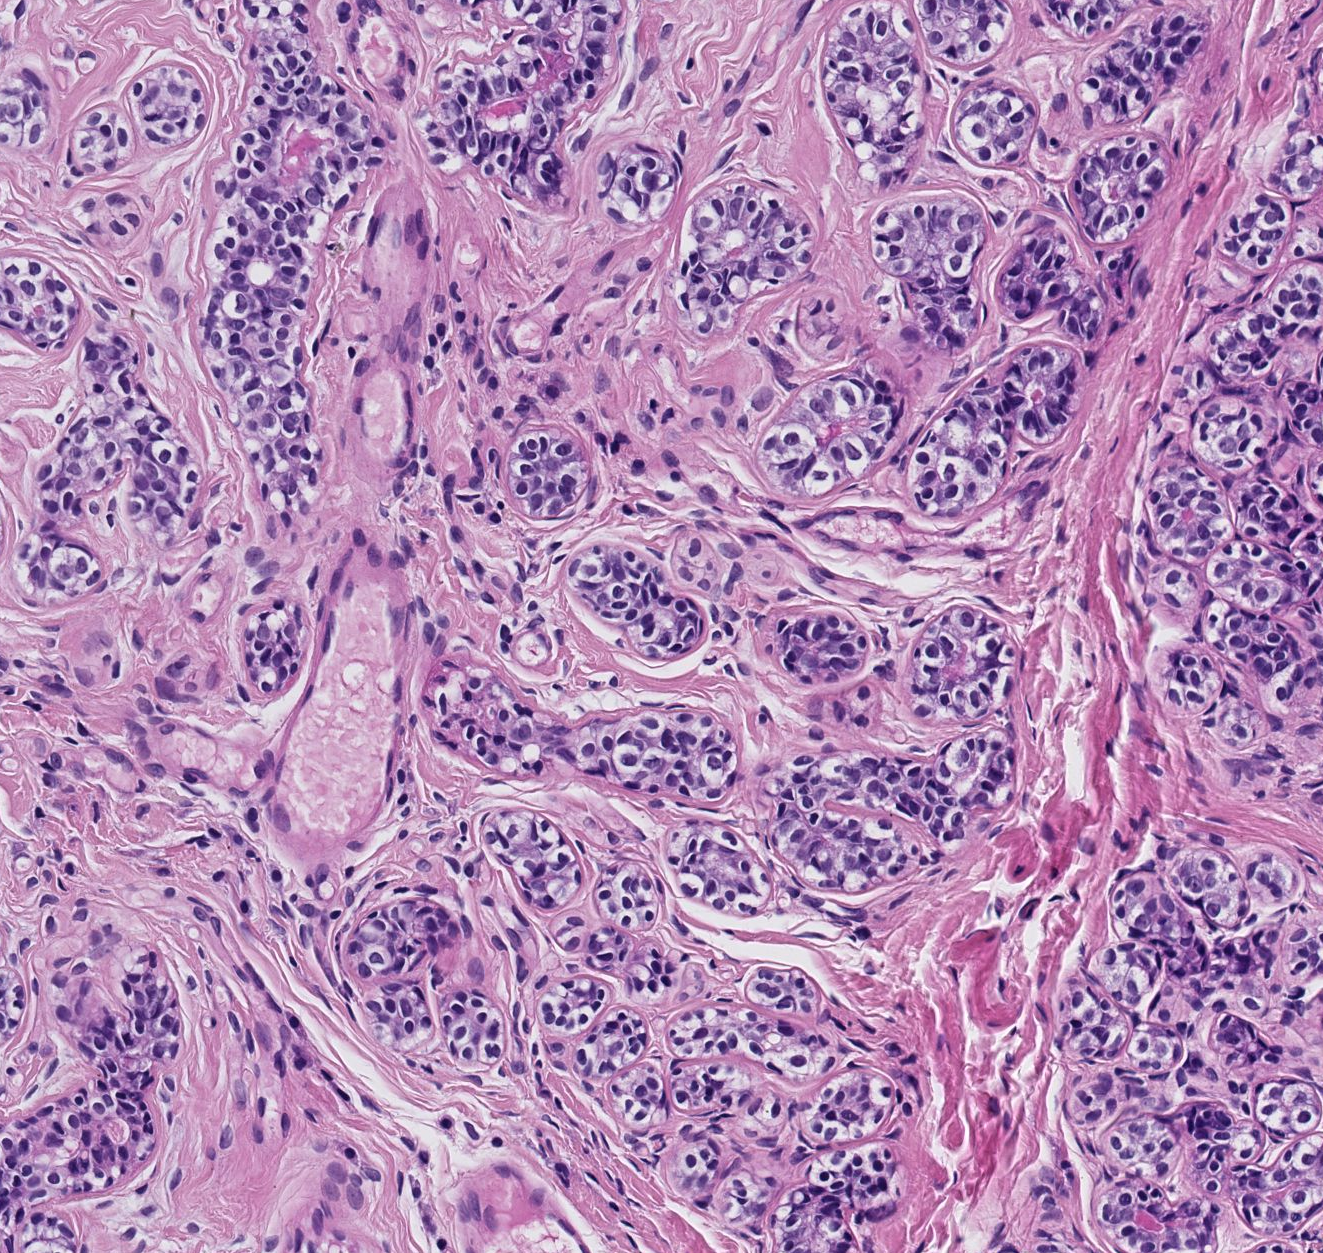
\includegraphics[width=8cm]{assets/images/histology_image_example.png}
\par\end{centering}
\caption{Example of histology image stained with haematoxylin and eosin \label{fig:h&e-image}}
\end{figure}

Slides stained by these chemicals are then examined by histopathology experts who try to identify key features which would determine a diagnosis, future treatment plan, or other subsequent steps. As a very good example of this whole process can serve a method of adjusting a treatment for patients who suffer from breast cancer.

\section{Motivation}

In recent decades breast cancer has been on of the leading causes of death among women and the second most commonly diagnosed type of cancer worldwide \cite{Bray2024, Siegel2023}. According to \cite{Bray2024} in 2022 breast cancer was attributing for approximately 2.3 million newly diagnosed patients - this represents 11.6\% of all diagnosed cancer patients in that year and 666,000 deaths, comprising 6.9\% of all cancer deaths. \cite{Siegel2023} informs that in the USA in the year of 2023 breast cancer among women accounted for more than 297,000 new cases - 31\% of all new female cancer cases and more than 43,000 deaths - 15\% of all female cancer deaths.

When dealing with breast cancer, one needs to keep in mind that there are also different subtypes of breast cancer. Firstly introduced in \cite{Perou2000}, we now know four breast cancer molecular subtypes, based on the positivity or negativity of several receptors. These receptors are Human Epidermal Growth Factor Receptor 2 (Her2) and Hormonal Receptor (HR), which is positive if either Estrogen or Progesterone receptors are positive; otherwise it is negative. These four classes along with respective receptor statuses can be seen in table \ref{tab:breast_cancer_subtypes}.

\begin{table}[H]
    \centering
    \caption{Breast Cancer Molecular Subtypes and Receptor Statuses}
    \label{tab:breast_cancer_subtypes}
    \begin{tabular}{|l|c|c|c|}
        \hline
        \textbf{Subtype Class} & \textbf{Hormone Receptor (HR)} & \textbf{Her2} \\
        \hline
        Luminal A & Positive & Negative \\
        \hline
        Luminal B & Positive & Positive \\
        \hline
        Her2-enriched & Negative & Positive \\
        \hline
        Triple Negative (TNBC) & Negative & Negative \\
        \hline
    \end{tabular}
\end{table}

From the aforementioned subtypes, the last three are the ones that currently have the worst prognosis \cite{Schalper2022, Zhang2024}. Identifying and using certain biomarkers could potentially improve the prognosis of patients with these subtypes of breast cancer. Tumour-infiltrating lymphocytes (TILs) appear as such biomarkers, especially their presence, number and spacial organization inside of the tumour and tumour-related tissue \cite{Salgado2015, Denkert2018, Amgad2019}.

However, manual identification and visual recognition of TILs from H\&E stained slides is a difficult, time-consuming, and error-prone task even when performed by experienced histopathology experts \cite{Salgado2015, Amgad2019}.

\section{Objectives}
Manual analysis of histopathology slides is expensive, takes long time to complete and requires highly trained professionals and quality assurance by performing peer reviews \cite{Wemmert2021}. With the invention of virtual microscopy, which enables H\&E stained glass slides to be converted into digital slides, and the introduction of Whole-slide Images (WSIs), the field is entering a new era. The term Digital Pathology or Digital Histopathology is often being used. In Digital Pathology, much effort is put into developing tools that would help medical experts to semi- or fully automate the visual analysis of the digital slides. Entities such as different tissue types and cells can be identified and classified.

Deep learning has shown extreme potential in many areas, including medicine and processing of medical image data \cite{LeCun2015}.

Usage of a deep learning models also introduces a new challenge: in order for them to lay reasonably good results, they need huge amount of high quality data \cite{Santosh2022-3}. Precise manual annotation of histology slides is not an easy nor a cheap task as we have mentioned earlier. Therefore, our aim in this work is to develop and implement a pipeline for automated detection and segmentation of tumour-infiltrating lymphocytes from breast cancer histology image slides using weak annotations, in the form of bounding boxes, of these cells. For this purpose we will be using the TIGER dataset, which is available via the Grand Challenge platform \cite{tiger_dataset}. Since the provided annotations of the TILs are in the form of bounding boxes, our goal is two-fold:

\begin{enumerate}
    \item Develop and implement effective and precise algorithm for creating pseudo-labels by converting bounding box annotations into pixel mask annotations.
    \item Implement and compare various deep learning architectures, e.g. U-net and its variants or Vision Transformer and select the best one based on the evaluation metrics such as Intersection over Union (IoU) and Dice coefficient.
\end{enumerate}

In the end, we want to have a model that will be able to effectively detect and segment individual cell nuclei from weakly annotated H\&E stained histology images of breast cancer patients.



% Chapter 1
\clearpage\null
\chapter{Computer Vision and Machine Learning}
Vision is one of our primary senses. Therefore, it is understandable that we seek methods for capturing, storing, analyzing, and processing this kind of data. Digital image processing is a vast area of different disciplines, ranging from low-level operations such as noise reduction, image sharpening, and contrast adjustment through mid-level operations like classification and segmentation to high-level operations which involve making higher sense of the images and resembling human visual perception and intelligence \cite{Gonzalez2018}. 

Computer Vision, a subfield of computer science and an extension of digital image processing focuses on using computers to extract meaningful knowledge from images in various ways, thereby emulating the capabilities of the human brain and visual cortex \cite{Gonzalez2018}. As part of machine learning and artificial intelligence, computer vision uses automation algorithms to analyze and process visual data, including 2D and 3D images as well as videos \cite{Szeliski2022, Atallah2020}.

Machine learning is a subset of artificial intelligence, which includes both statistical learning and deep learning algorithms to make intelligent decisions based on data. Modern computer vision primarily utilizes deep learning techniques, as illustrated in figure \ref{fig:ai-ml}. In classical programming, we are designing an explicit program that produces desired outputs for specific inputs. In machine learning, however, we let the machine design an appropriate program, given the specified set of inputs and outputs (labels) by analyzing the features and patterns of the input with relation to the output \cite{Alam2021}.

\begin{figure}[H]
\begin{centering}
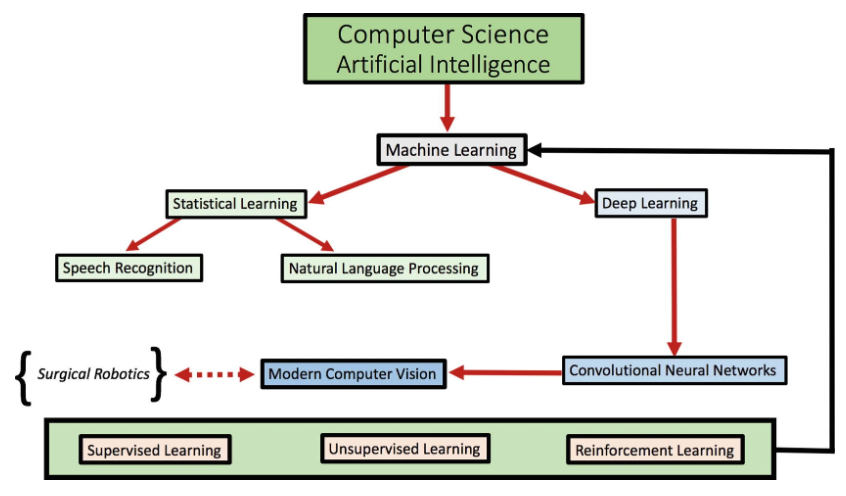
\includegraphics[width=12cm]{assets/images/aiml.png}
\par\end{centering}
\caption{Division of AI/ML \cite{Atallah2020}}
\label{fig:ai-ml}
\end{figure}

With the advent of deep learning \cite{LeCun2015} and especially convolutional neural networks \cite{Ronneberger2015}, computer vision is now a field of huge interest.

\section{Preprocessing}
Since the machine learning algorithms try to examine the relationship between input and output, we need to ensure an appropriate quality of the input data. Especially in medical imaging and digital histopathology, where the different staining techniques, scanning tools, or position of the tissue can vary widely and this can have an effect on the further analysis \cite{Hoque2024}.

In the domain of digital histopathology, a common issue are the varying intensities of purple, red, and pink tones of H\&E stained slides \cite{Hoque2024}. For this purpose, different stain normalization techniques were created. Among the examples, we can list the Macenko, Reinhart, or Zheng normalization techniques, which try to normalize the dataset of input images \cite{Hoque2024}. Among some other techniques, we can list the histogram equalization, Contrast-Limited Adaptive Histogram Equalization (CLAHE), and the power law (gamma) transformation \cite{Dabass2020}.

\section{Core Computer Vision Tasks}
When analyzing an image, we can come across the three main tasks \cite{Alam2021}. The example of each of these tasks can be seen in figure \ref{fig:aiml-tasks}.

\begin{figure}[H]
\begin{centering}
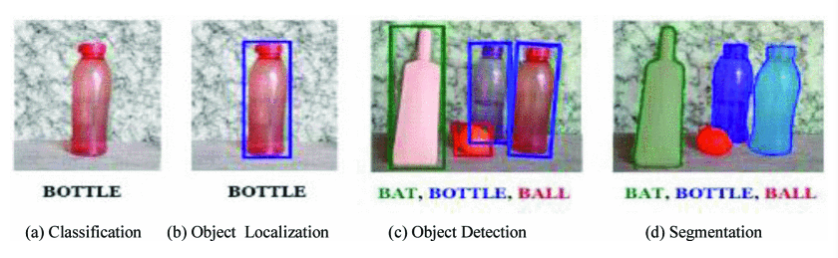
\includegraphics[width=12cm]{assets/images/aiml-tasks.png}
\par\end{centering}
\caption{Different Computer Vision tasks \cite{Alam2021}}
\label{fig:aiml-tasks}
\end{figure}

\subsection{Image Classification}
Image classification is used when we have a label categorizing the image into one of the classes (or multiple classes) in the set of classes \cite{Alam2021}. For example, in the medical imaging domain, we could label an image with the "disease" or "non-disease" class.

\subsection{Object Localization and Object Detection}
Object localization and object detection are very similar tasks. While the former is a task of localizing a single object instance in the image, the latter is a task where multiple instances of one or many objects should be detected and bounded \cite{Alam2021}.

\subsection{Segmentation} Sometimes we want to get a more detailed label than just an approximate object location (bounding rectangle). Segmentation utilizes pixel-level classification, where pixels can be labeled based on their relationship to various classes. According to \cite{Alam2021} we know two main types of segmentation:

\begin{itemize}
    \item Semantic segmentation, where each pixel of a certain class gets the same label, no matter the number of instances, and
    \item Instance segmentation, where the pixels of different instances of the same class are distinguished as well.
\end{itemize}

Apart from the currently most popular and interesting segmentation algorithms using deep learning, we also know some traditional segmentation techniques, like the GrabCut algorithm.

The GrabCut algorithm was first introduced in \cite{Rother2004} as a foreground extractor. With it, we are able to segment a foreground object and isolate it from the background. The GrabCut takes an image as an input, with a tight rectangular label indicating where the object we want to segment is located. Everything outside of this region is considered background and everything inside of this region is unknown. A user can hard-label parts of this region to explicitly indicate that those pixels belong to either foreground or background. Then a Gaussian Mixture Model models the the foreground and background regions. It utilizes color statistics to label unknown pixels as probable foreground or probable background. Next, a graph is created from these pixels, where each pixel represents a single node in the graph. In addition to pixel nodes, the source and the sink nodes are added to the graph. All foreground pixels are connected to the source node and similarly, all background pixels are connected to the sink node. The weights on the edges of the pixels that are connected both to the source and the sink node are defined by the probability of the pixel being either foreground or background. The edge information or the pixel similarity is used to define the weight on the edges between the pixels. Finally, a mincut algorithm processes the graph to separate the source and sink nodes. In the end, every pixel that is connected to the source node is labeled as foreground and every pixel connected to the sink node is labeled as background \cite{opencv_grabcut}.


\section{Learning Paradigms}
Computer vision algorithms can be further divided by how they can learn from the data \cite{Alam2021}.

\paragraph{Supervised Learning} In the supervised learning tasks, both the data and their respective labels are known and are available to the model during the training. Typical supervised learning tasks include classification, detection, and segmentation. By the quality and precision of the labels and the task goal, we can split supervised learning into three categories:

\begin{itemize}
    \item Standard supervised learning, when available labels are of the same quality as the labels we want to predict, e.g. bounding box to bounding box.
    \item Strong supervised learning, when the training labels contain richer information than the labels we want to predict, e.g. bounding box from pixel-level annotations.
    \item Weak supervised learning, when the training labels contain less precise information than the labels we want to predict, e.g. bounding box from image level annotation.
\end{itemize}

\paragraph{Unsupervised Learning} In unsupervised learning, on the other hand, the data labels are not available to the model during the training.


% Chapter 2
\clearpage\null
\chapter{Deep Neural Networks}

The history of artificial neural networks (ANN) dates back to 1943. In \cite{McCulloch1943} authors tried to mathematically describe the activity of biological neurons in the human brain. Using these principles they built a first artificial neuron and artificial neural network. In 1974 a PhD student, Paul Werbos, introduced in \cite{Werbos1974} the idea of backpropagation of errors by which ANN are able to learn other than linearly separable problems, and this idea was further expanded in \cite{Rumelhart1986}. Artificial neural networks that contain many hidden layers are also called deep neural networks (DNN) and the process of training this network is called deep learning \cite{LeCun2015}. Over the years deep learning and one of its variants - convolutional neural network that was proposed in \cite{LeCun2015-2} - were found to be very effective and precise in domains that were found unreachable by the classical AI and ML algorithms \cite{LeCun2015}. This was caused by their ability to capture abstract and complex patterns that simpler models found impossible to catch. Such examples include analysis of image data \cite{Farabet2013, Alzubaidi2021} and recent advancements in natural language processing (NLP) \cite{Deng2018}.

\section{Structure}
The fundamental part of every artificial neural network is the neuron. Neuron is basically a function which has one or more inputs and one output. Inside of this neuron, a mathematical computation is being done in order to transform input into output. Input can also be referred to as input vector or vector of input features. Each input feature has its weight by which it is multiplied. Next a bias is added to the multiplied and summed features and weights. This calculation is still linear so in order for it to be able to capture more complex patterns, we need to apply non-linear activation function to its output. The mathematical representation of artificial neuron can be seen in the equation bellow:

\begin{align}
    z &= b + \sum_{i=1}^n (w_i x_i) \\
    a &= f(z)
\end{align}

Where $z$ is the output produced by the linear unit, $b$ is the bias, $n$ is the number of input features, $x_i$ is the \textit{i}-th input feature, $w_i$ is the weight associated with the \textit{i}-th input feature, $a$ is the actual output, and $f$ is the activation function.

Visual example of artificial neuron can be seen in figure \ref{tab:artificial-neuron}.

\begin{figure}[H]
\begin{centering}
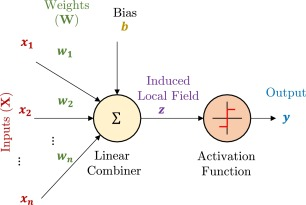
\includegraphics[width=8cm]{assets/images/neuron.jpg}
\par\end{centering}
\caption{Artificial neuron \cite{Santosh2022-1}}
\label{tab:artificial-neuron}
\end{figure}

\subsection{Activation Functions}

\subsection{Layers}

Similarly to biological neural networks, when artificial neurons are chained together, meaning the output from one neuron is passed to another neuron, they create an artificial neural network.

This network is organized in layers. Neurons in each layer are not connected together, but rather every neuron from layer \textit{L} is connected with every neuron from layer \textit{L+1}, except neurons in the first (input) layer. For better understanding, we will refer to the figure \ref{tab:artificial-nn} where we can see an example of a neural network.

\begin{figure}[H]
\begin{centering}
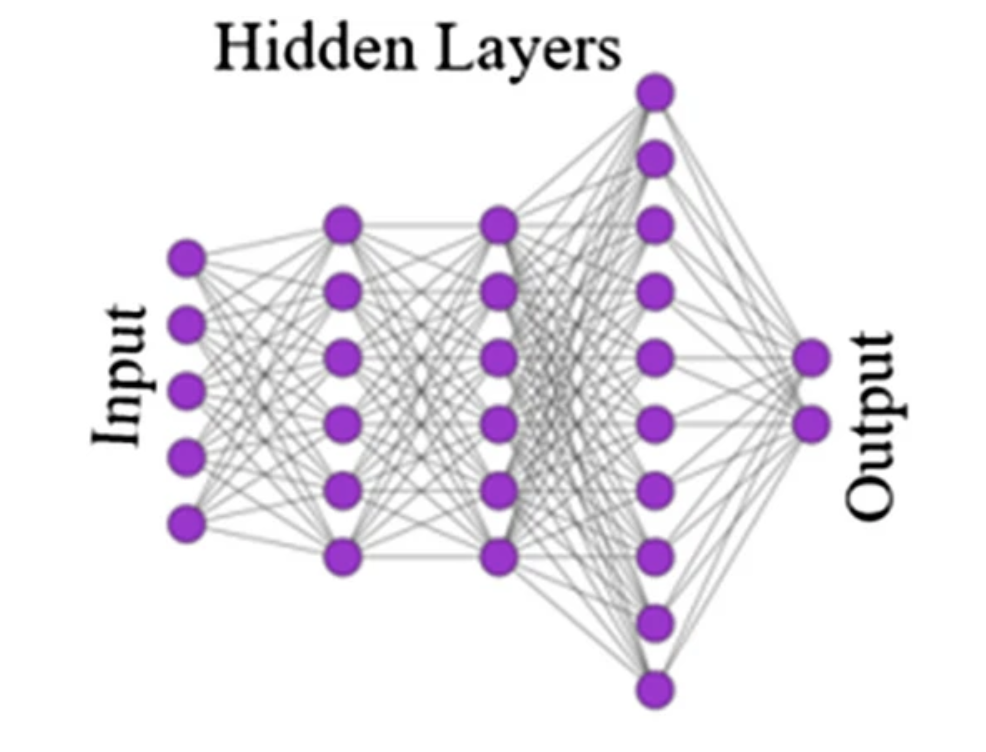
\includegraphics[width=8cm]{assets/images/neural_net.png}
\par\end{centering}
\caption{Example of deep artificial neural network \cite{TalaeiKhoei2023}}
\label{tab:artificial-nn}
\end{figure}

Neural network can be split into three main parts:

\begin{itemize}
    \item An input layer
    \item Hidden layers
    \item Output layer
\end{itemize}

Input layer is the initial layer and the only layer that does not contain neurons which perform calculations but rather consists of \textit{N} input features $x_1, x_2, \dots, x_N$ also referred to as a vector $\vec{x}$ of input features:

\[
\vec{x} = \begin{bmatrix}
x_1 \\
x_2 \\
\vdots \\
x_N
\end{bmatrix}
\]

The subsequent layers between the input layer and output layer are called hidden layers. The name comes from the fact that their outputs are not directly observable, nor are they provided by the external environment - they are internal to the network's architecture. Neurons inside these layers perform calculations on the input and produce output, which is then fed forward to the next layer.

The final output layer produces an output of the network. Output and number of neurons depend on the task the network is being trained for. For regression task one neuron is often suitable - it predicts a continuous variable \cite{Goodfellow2016}. During classification task it can further depend on the nature of the classification. In binary classification, again a single neuron can suffice. It will display a probability of the input belonging to one of the classes - if the probability is high, it will assign that class to it, and if the probability is low, it will assign the other class to it \cite{Goodfellow2016}. In multi-class classification, the number of neurons is the same as the number of classes and each neuron predicts a probability of the input belonging to one specific class \cite{Goodfellow2016}.

%TODO: input, hidden, output layer, deep nn, image

\section{Loss Functions}

\section{Training}

\subsection{Forward Propagation}

\subsection{Backpropagation}

\subsection{Hyperparameters}

\section{Evaluation Metrics}

\section{Architectures}

% Chapter 3
\clearpage\null
\chapter{Deep Learning in Digital Histopathology}
Manual analysis of histopathology slides is expensive, takes long time to complete and requires highly trained professionals and quality assurance by performing peer reviews \cite{Wemmert2021}. With the invention of virtual microscopy, which enables glass slides to be converted into digital slides, and the introduction of Whole-Slide Images (WSIs), the field is entering a new era. The term Digital Pathology is often being used. In Digital Pathology, much effort is put into developing tools that would help medical experts to semi- or fully automate the visual analysis of the digital slides. Entities such as different tissue types and cells can be identified and classified.

Deep learning has shown extreme potential in many areas, including medicine and processing of medical image data \cite{LeCun2015}.

\section{Architectures}
Neural network architectures like Convolutional Neural Networks \cite{LeCun2015-2} and U-Net \cite{Ronneberger2015} have proven to be effective in medical image analysis \cite{Santosh2022-2}. In recent years, also a concept of Vision Transformers \cite{Dosovitskiy2020, Hu2023} used in medical imaging shows promising results \cite{Shamshad2023, Hu2023, He2023}.

\subsection{Convolutional Neural Networks}

\subsection{U-Net}

\subsection{Vision Transformer}

\section{Challenges, Strategies and Future Directions}

\subsection{Data Annotation}

\subsection{Weakly Supervised Learning}

\subsection{Active Learning}

\subsection{Future Trends}



% ----- IN FINAL WORK -----
% Evaluation
%\clearpage\null
%\chapter{Evaluation \label{cha:eva}}


% -------------------------

% Related Work
\clearpage\null
\chapter{Related Work}
Precise manual cell annotation on huge WSI slides is a laborious task that needs to be performed by skilled expert pathologists. There exists a large number of models trained on the pixel-level masks for cell segmentation, which perform remarkably well. In the field of weak supervision for cell segmentation, a number of studies focus either on weak supervision in the form of point annotations in H\&E slides, or weak supervision with bounding box annotations of cells in microscopic imaging or DNA cytometry. However, we did not find many studies focusing on weakly annotated cell segmentation, especially from the histopathological H\&E stained slides, when annotations were presented in the form of bounding boxes. Therefore, to comprehensively review the current state of research, we will first examine studies that utilize bounding box cell annotations in histology. Subsequently, we will explore selected papers focusing on cell annotations using bounding boxes in modalities other than histology, as well as those addressing weakly supervised cell segmentation in histology employing point annotations of cell nuclei.

% short intro, what they do and propose, findings, modalities
% dataset and labels
% methodology (architecture + image)
% results and metrics (tables)

\section{Guided Prompting in SAM for Weakly Supervised Cell Segmentation in Histopathological Images \cite{Tyagi2023}}
The authors of this work explore the applicability of the Segment Anything Model (SAM), using guided prompting, to the cell segmentation task from histology image slides, where the cells are only annotated using bounding box labels. Their results outperformed other models for weakly supervised segmentation by a huge margin.

Three different datasets were used, and since each dataset was annotated with pixel-level masks, these were converted into the bounding boxes for the purpose of this study and the segmentation mask labels were not used during the training. If the dataset also contained class labels for individual cell nuclei, these labels were not used as this study is not concerned with cell classification. The datasets used were: 

\begin{enumerate}
    \item ConSep dataset, containing 41 H\&E stained WSIs, each having $1000\!\times\!1000$ pixels. The images are of single cancer and colorectal adenocarcinoma. Together there are 24,319 annotated cells, split into three different categories (inflammatory, epithelial, spindle). For the purpose of this work, each image was split into four patches, each patch having $500\!\times\!500$ pixels. Then 98 of these patches were used for training, 10 for validation, and 56 for testing.
    \item MoNuSeg is a multi-organ cell segmentation dataset containing 51 H\&E stained images of different organ tissue (stomach, bladder, breast, liver, kidney, prostate, colon). Together the images have 28,846 annotated cell nuclei. Similarly to the ConSep, each $1000\!\times\!1000$ image is split into four $500\!\times\!500$ patches, 133 of them used for training, 15 for validation, and 56 for testing.
    \item TNBC dataset of 50 $512\!\times\!512$ WSIs of triple-negative breast cancer tissue. In total, it contains 4,022 annotated cell nuclei. 34 images were used for training, 5 for validation, and 11 for testing.
\end{enumerate}

Two main approaches were used. During the first, called D-SAM, a YOLO object detector was trained to generate the bounding boxes of cells, using a sum of three losses (objectness loss - $\mathcal{L}_{obj}$, classification loss - $\mathcal{L}_{cls}$, and localization loss - $\mathcal{L}_{loc}$). During the inference (the testing, at the time of prediction) the image along with bounding boxes predicted by the detector model were embedded and fed to the SAM to predict the segmentation masks (with bounding box predicted labels as guiding prompts). The second approach, called SAM-S, used SAM as a pseudo-label generator. Both images and corresponding ground truth labels were embedded and fed to the SAM and its output segmentation masks were then used as pseudo-labels to train a separate segmentation model with combined Dice loss ($\mathcal{L}_{dice}$) and binary cross entropy ($\mathcal{L}_{BCE}$). Both approaches can be seen in figure \ref{fig:rw-sam}. 

\begin{figure}[H]
    \begin{centering}
    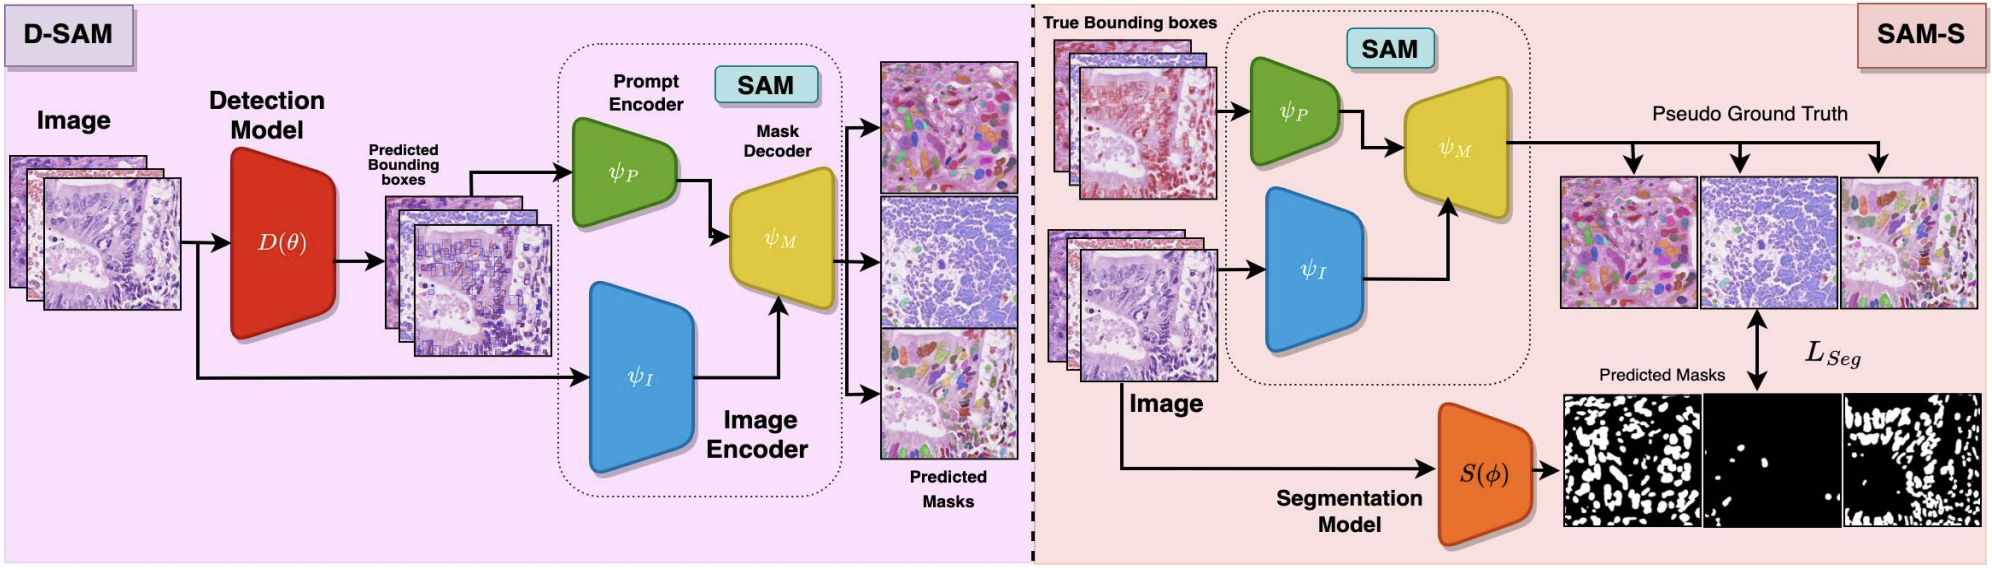
\includegraphics[width=14cm]{assets/images/rw-sam.png}
    \par\end{centering}
    \caption{Workflows with SAM \cite{Shamshad2023}}
    \label{fig:rw-sam}
\end{figure}

In addition to these, three more strategies were used, namely:

\begin{enumerate}
    \item SAM-W, where SAM was fine-tuned using weakly supervised losses
    \item SAM-M, where the mask generated by the SAM-S approach is used as a guiding prompt for another SAM prediction
    \item SAM-ILP, where an Integer Linear Programming is used as a post-processing technique to align the results obtained both from the D-SAM and SAM-S approaches
\end{enumerate}

Different prompting methods were used and also a no-prompting case, where only an image was provided was used. In the 1P-\textit{k}N scenarios, one positive and \textit{k} negative points were used for each bounding box, where the positive point was the center of the bounding box and negative points were outside of the bounding box and were not part of any other bounding box. All of the prompting methods are summarized in figure \ref{fig:rw-sam-prompting}, where we can see that the bounding box prompts achieved the best Dice scores in most cases.

\begin{figure}[H]
    \begin{centering}
    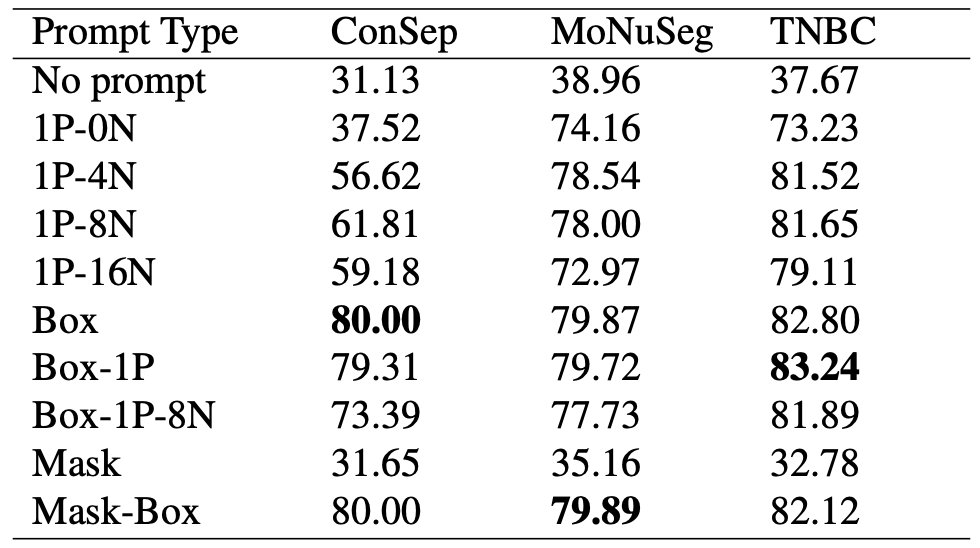
\includegraphics[width=8cm]{assets/images/rw-table-prompting.png}
    \par\end{centering}
    \caption{Different prompting methods used for SAM}
    \label{fig:rw-sam-prompting}
\end{figure}

Mean average precision (mAP), precision, and recall were used as evaluation metrics for object detection, and the Dice coefficient was used as an evaluation metric for segmentation.

Two non-SAM models were used as baselines for comparison, the BBTP and BB-WSIS, both based on the Residual U-Net architecture, trained for 50 epochs and a learning rate of 0.0001. Yolov8x was used as the object detector, trained for 300 epochs with early stopping, batch size 32, and decreasing learning rate (starting at 0.01 and decreasing by a factor of 10). The CaraNet was used as the segmentation model. It uses reverse axial attention and has great performance for small objects. It was trained for 200 epochs, with Adam optimizer, learning rate 0.0001, and early stopping. The experiments were carried out using NVIDIA-RTX 5000 and Tesla A100 GPUs.

From the results displaying the Dice scores shown in figure \ref{fig:rw-sam-dice} we can see that both SAM-S and D-SAM outperformed the baseline models and the overall best results were achieved by the SAM-ILP model.

\begin{figure}[H]
    \begin{centering}
    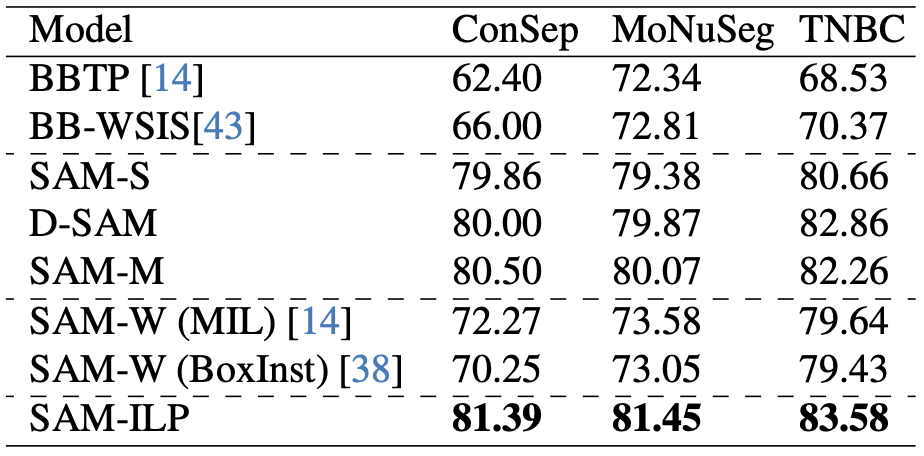
\includegraphics[width=8cm]{assets/images/rw-table-dice.png}
    \par\end{centering}
    \caption{Comparison of used models with Dice scores}
    \label{fig:rw-sam-dice}
\end{figure}

\section{A pathomic approach for tumor-infiltrating lymphocytes classification on breast cancer digital pathology images \cite{Verdicchio2023}}
The second study aimed to classify TILs in H\&E stained images of breast cancer based on the handcrafted set of features, to achieve a better model explainability. Even though the main focus of this study is different from our goals, it is relevant and interesting for us for two reasons:

\begin{enumerate}
    \item it uses the same TIGER dataset \cite{tiger_dataset} as we do, and
    \item it uses a watershed-based method to segment cell nuclei within the tissue as a preprocessing step.
\end{enumerate}

The dataset contains 195 WSIs scanned at three different institutes. They contain region of interest (ROI) annotations of both tissue types and TILs. TILs were annotated using point annotations and a bounding box of $8 \!\times\! 8$ \textmu m was constructed and centered on the point.

In the preprocessing step, the authors applied a stain normalization proposed in \cite{Vahadane2015}, and watershed-based cell nuclei segmentation. The authors decided to use this method for its simplicity, speed, and easy parameter adjustments and fine-tuning. The method used mathematical operations. They used the implementation from the QuPath digital pathology tool with the following set of parameters:

\begin{itemize}
    \item The setup parameter: hematoxylin OD for the detection image, pixel size of 0.5\textmu m
    \item Nucleus parameters: background radius $8 \text{\textmu m}$; median filter radius $0 \text{\textmu m}$; $\sigma = 1.5 \text{\textmu m}$; minimum cell area $10 \text{\textmu m}^2$; maximum cell area $400 \text{\textmu m}^2$
    \item Intensity parameters: threshold 0.1; maximum background intensity 2
\end{itemize}

The resulting segmentation masks were verified by an expert microscopist. This method was applied to 1037 ROIs, where 92,141 cell nuclei were segmented; 20,111 of them being TILs.

The study further worked on the TIL/non-TIL classification task and identifying the relevant features, but since this is not our primary interest, we only briefly describe the methodology and results. The study analyzed 71 features split into five groups (6 Fourier Shape Descriptors features - FSD, 8 gradient features, 26 Haralick features, 12 intensity-based features, 19 morphometry features). Out of them, 21 were selected as patomic features. These should best describe the properties of TILs. Then five different classification models (Random-Forest, Decision Tree, Linear Discriminant Analysis, K-Nearest Neighbors, Multi-layer Perceptron) with three different resampling techniques (none, synthetic minority oversampling technique - SMOTE, Down) were trained using these features. The AUC (area under the ROC curve), accuracy, precision, sensitivity, specificity, and F1-score were used as evaluation metrics. The Random-Forest classifier achieved the best result with an AUC of 0.86, where the resampling technique did not make a significant difference.

\section{DDTNet: A dense dual-task network for tumor-infiltrating lymphocyte detection and segmentation in histopathological images of breast cancer \cite{Zhang2022}}
The third work introduces a dense dual-task network (DDTN), which is used both for TIL detection and segmentation in breast cancer H\&E stained images using only point annotations. These two modules share the same backbone, which allows them to learn from one another and promote each other. The ultimate goal of this network is to perform a precise TIL instance segmentation.

The training and testing workflows of the network can be seen in figures \ref{fig:rw-ddtn-train} and \ref{fig:rw-ddtn-test}. During the training phase, the network produces three output types for cells - bounding boxes, cell contours, and cell masks. The separate semi-automatic tool is used to create segmentation masks, from which bounding boxes and cell contours are derived. These are then used to guide the training of the model. During the inference phase, a network is used to produce the aforementioned three types of output again. Cell masks and contours are then unified to create cell segmentation masks and these are further merged with the detection bounding boxes to provide the final output.

\begin{figure}[H]
    \begin{centering}
    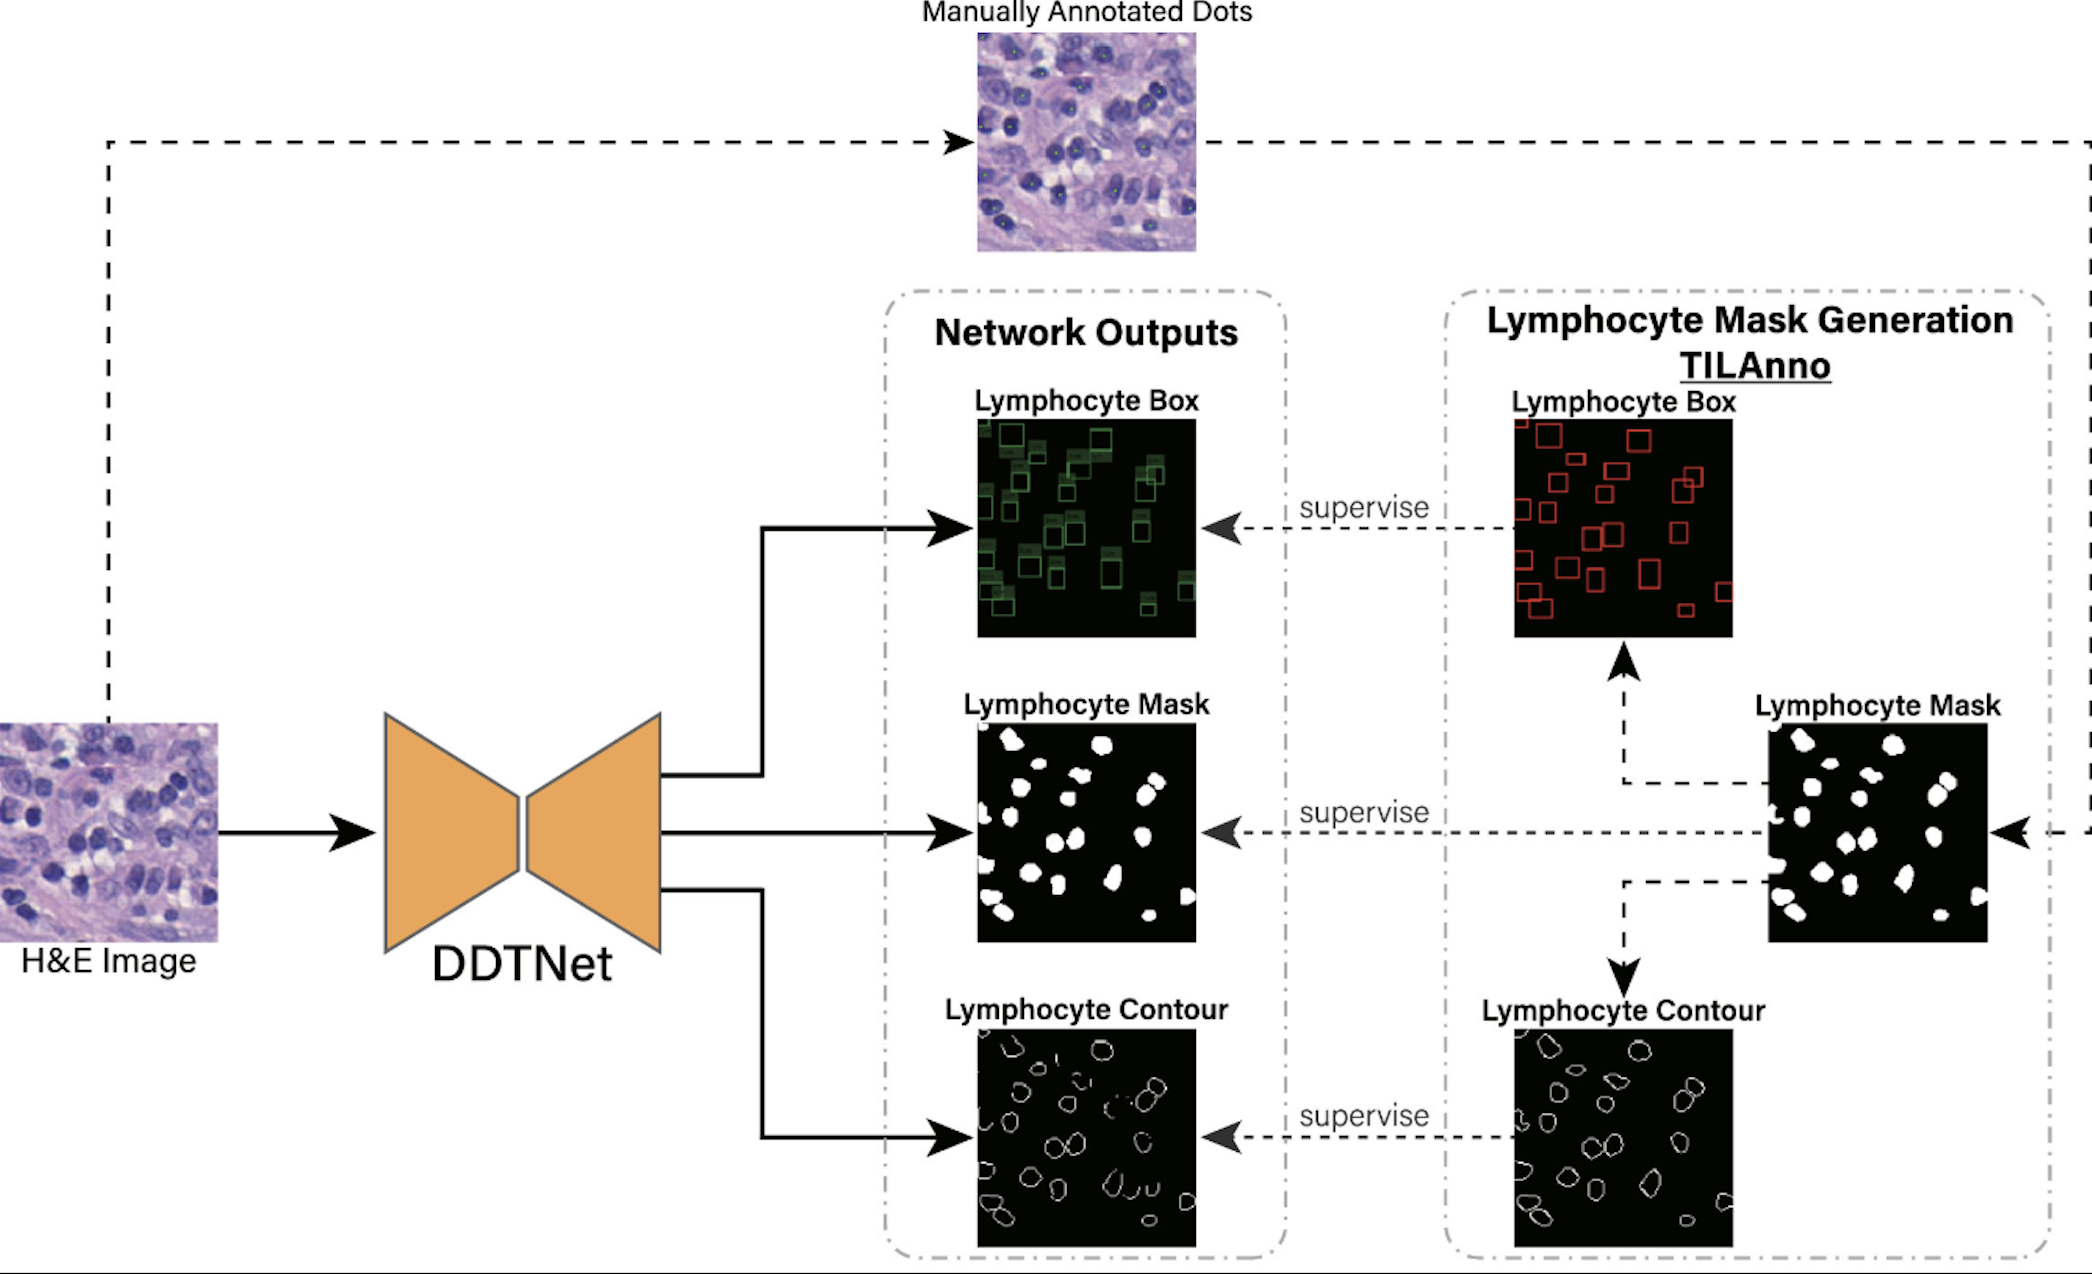
\includegraphics[width=12cm]{assets/images/rw-ddtn-train.png}
    \par\end{centering}
    \caption{DDTN workflow during training}
    \label{fig:rw-ddtn-train}
\end{figure}

\begin{figure}[H]
    \begin{centering}
    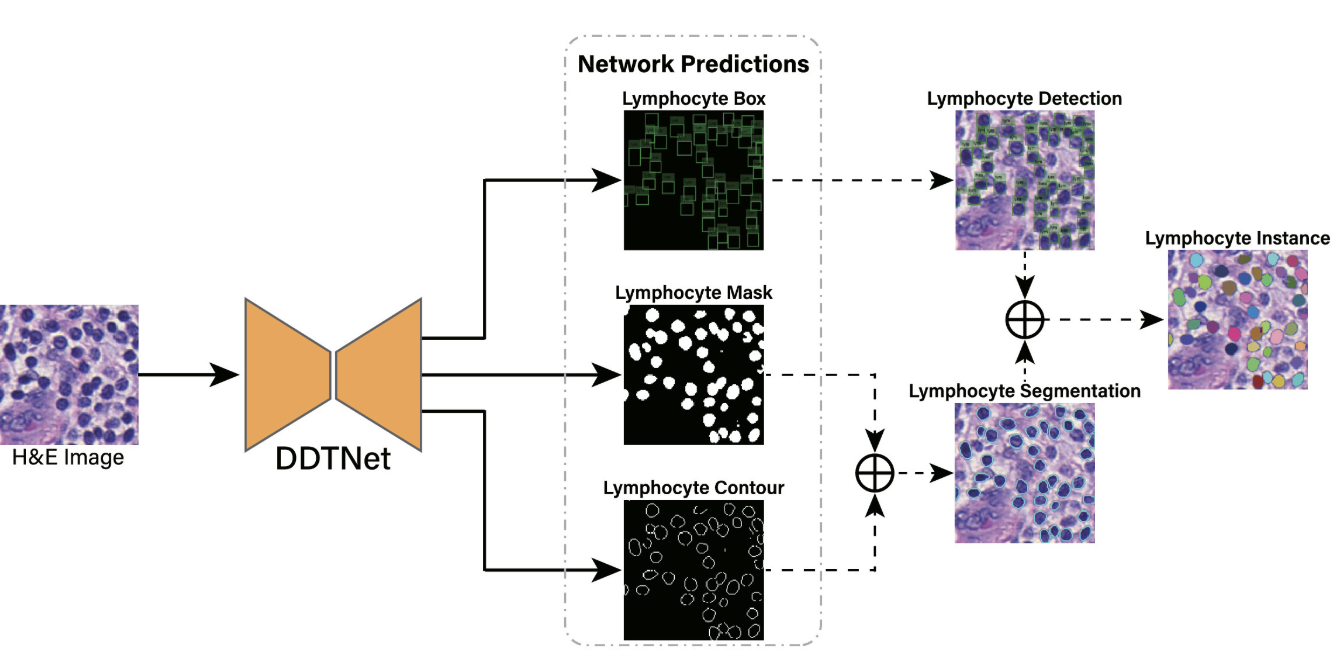
\includegraphics[width=12cm]{assets/images/rw-ddtn-test.png}
    \par\end{centering}
    \caption{DDTN workflow during inference}
    \label{fig:rw-ddtn-test}
\end{figure}

A detailed architecture of the DDTN model and each of its key components, like the backbone model, segmentation and detection modules, and feature fusion module can be seen in figure \ref{fig:rw-ddtn-arch}.

\begin{figure}[H]
    \begin{centering}
    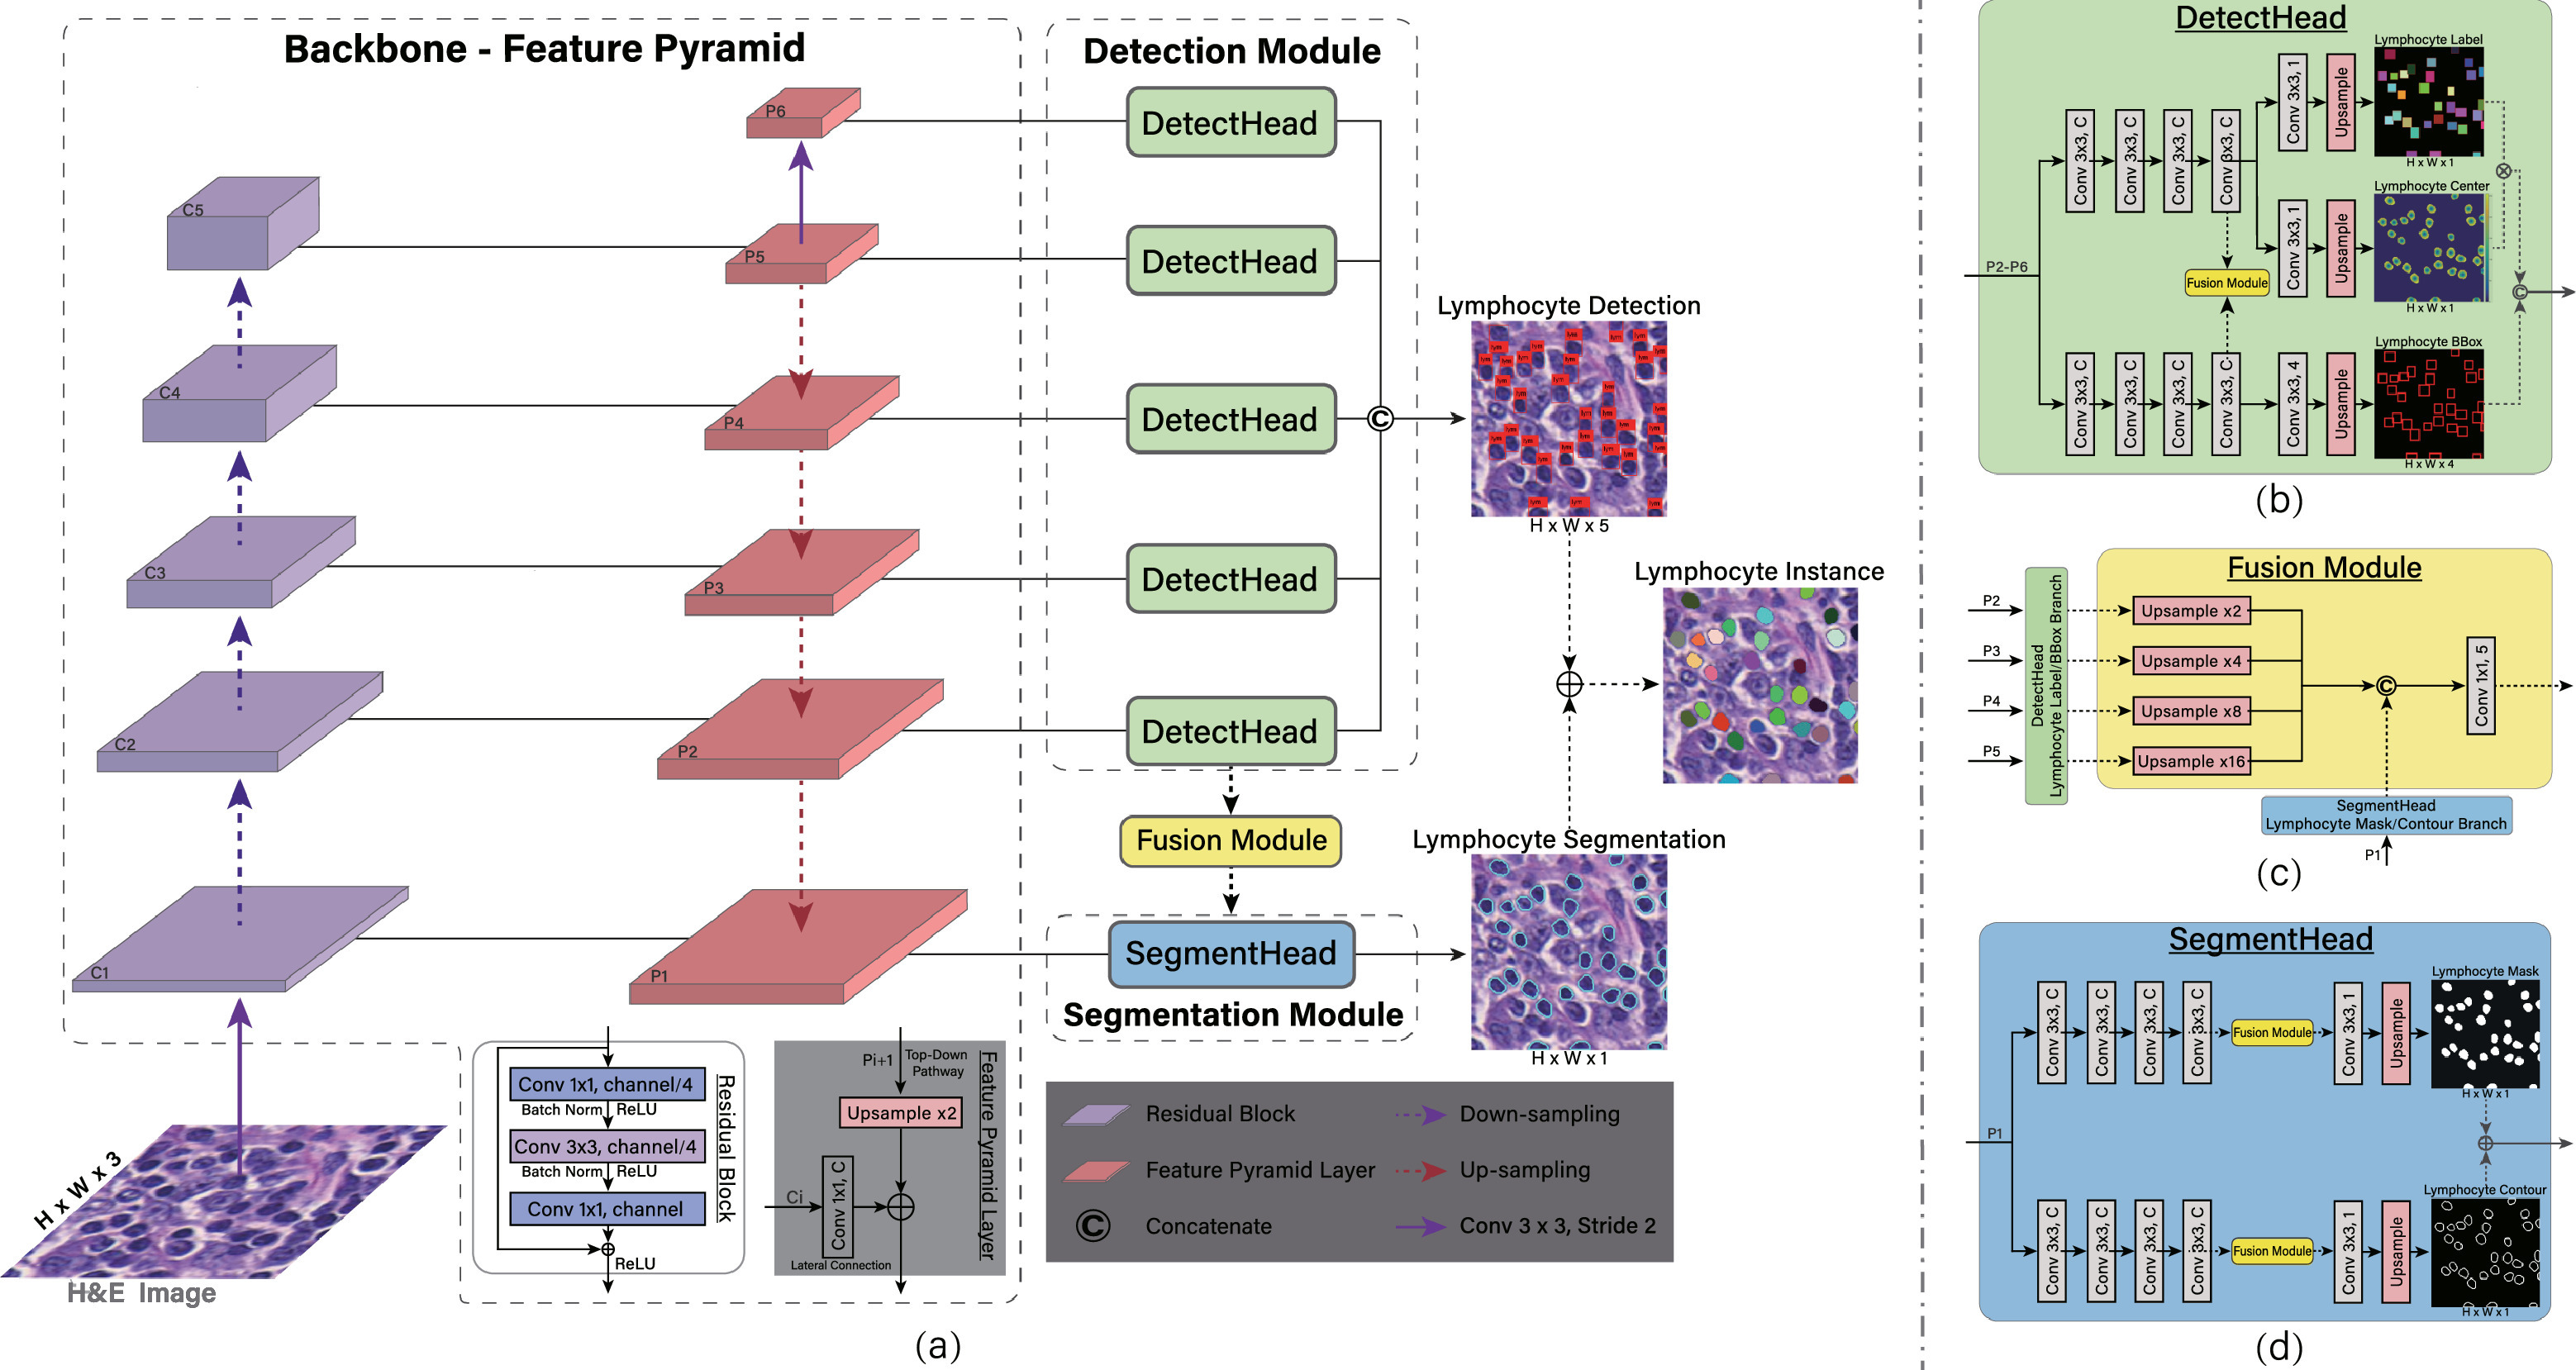
\includegraphics[width=14cm]{assets/images/rw-ddtn-architecture.jpg}
    \par\end{centering}
    \caption{DDTN architecture}
    \label{fig:rw-ddtn-arch}
\end{figure}

The study uses two publicly available datasets and creates a new one with the use of their semi-automatic mask generator, which the authors called TILAnno. The datasets used were:

\begin{itemize}
    \item BCa-lym dataset: containing 100 H\&E stained ROIs of size $100\!\times\!100$ pixels. 3,064 cells with point annotations are present on them.
    \item Post-NAT-BRCA dataset: contains H\&E stained WSIs with manual annotations of different cell types. For the purpose of this study, 29 WSIs were selected and 740 ROI patches of size $100\!\times\!100$ pixels were used, together containing 4,488 dot-annotated lymphocytes.
    \item TCGA-lym introduced dataset: authors used 15 H\&E stained WSIs from The Cancer Genome Atlas (TCGA), extracted ROIs of size $1600\!\times\!1600$ and let two junior pathologists annotate the lymphocyte centers and then a single expert refined them. In total 5,029 cells were annotated. For the training, each ROI was divided into 64 $200\!\times\!200$ patches.
\end{itemize}

Each dataset originally contained dot annotations of lymphocytes. The authors used the TILAnno tool to generate pixel-level masks, contours, and bounding boxes.

During the training, the input images were firstly resized to $320\!\times\!320$ pixels, and different augmentation techniques were used (mirror, flip, light noise, brightness, and color conversion). ResNet101 was used as a backbone network and it was pre-trained on the ImageNet dataset. The training hyperparameters were set in the following fashion: 1000 epochs with stochastic gradient descent, batch size of 4, an initial learning rate of 0.0001, and decreased by a factor of 10 at the 500th and 750th epochs; weight decay was set to 0.01 and momentum to 0.9.

Evaluation metrics were split for detection and segmentation tasks. In the lymphocyte segmentation task, the Dice score, Aggregated Jaccard Index, and panoptic quality were used. In the lymphocyte detection task, the precision, recall, and F1-score were used, where the truthfulness of the positivity of a sample was determined by the IoU threshold set to 0.5 in case of TP/FP and FN if the bounding box does not interest any ground truth bounding box.

For the evaluation of the TILAnno tool, the authors compared it to two other tools used for weak cell segmentation, namely QuPath and Cell Profiler. They ran all three tools on all three datasets, then let two experts manually label lymphocyte boundaries on 20 randomly selected images, which were used for evaluation with expert labels as ground truth. The TILAnno tool (Ours) seemed to outperform the baseline tools by a great margin in the Dice score as can be seen in figure \ref{fig:rw-ddtn-tilanno}. The study further analyzed the model performance of their proposed solution with other baseline models during inference, and from figure \ref{fig:rw-ddtn-results} we can see that their model outperformed them in all metrics except time.

\begin{figure}[H]
    \begin{centering}
    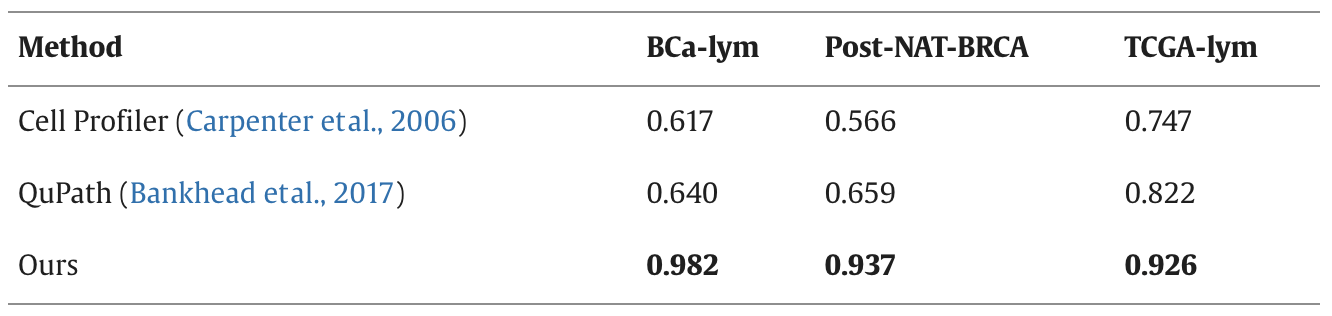
\includegraphics[width=14cm]{assets/images/rw-ddtn-tilanno-eval.png}
    \par\end{centering}
    \caption{Comparison of TILAnno and baseline tools}
    \label{fig:rw-ddtn-tilanno}
\end{figure}

\begin{figure}[H]
    \begin{centering}
    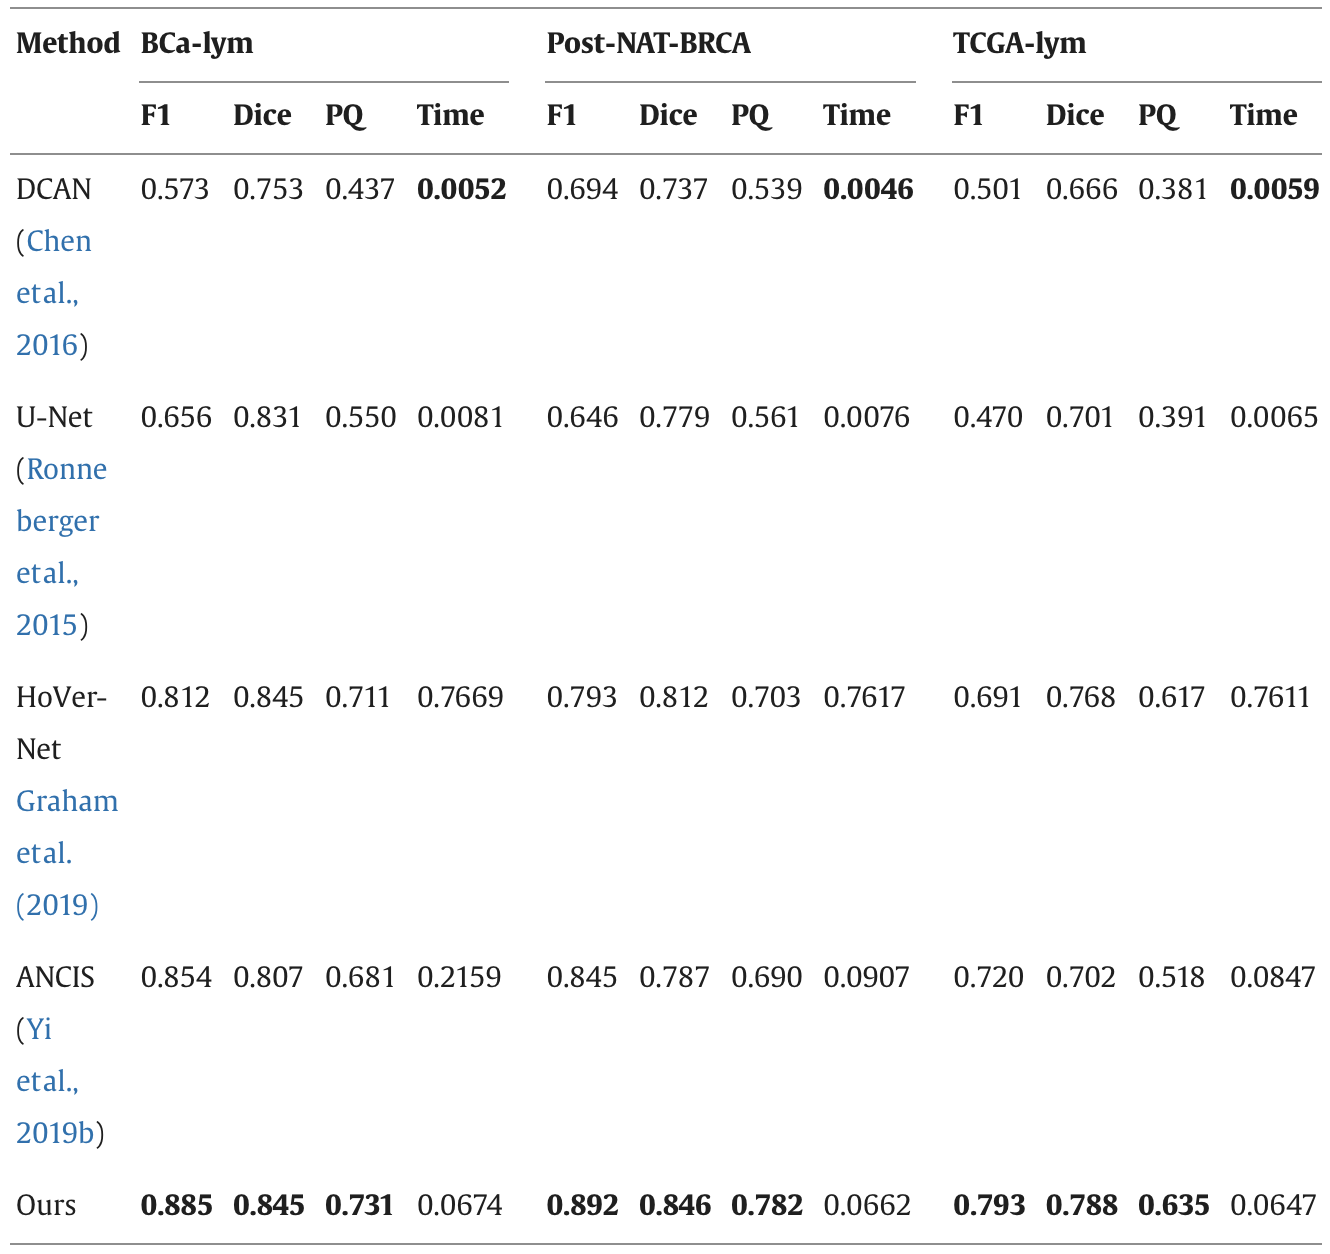
\includegraphics[width=14cm]{assets/images/rw-ddtn-results.png}
    \par\end{centering}
    \caption{Comparison of DDTN and baseline models}
    \label{fig:rw-ddtn-results}
\end{figure}

Moreover, the study also evaluated the model's ability to generalize, by training it only on the BCA-lym and Post-NAT-BRCA datasets and evaluating it on the TCGA-lym dataset. The results are summarized in figure \ref{fig:rw-ddtn-generalize} where we can see that their model again outperformed the existing baselines in all used metrics.

\begin{figure}[H]
    \begin{centering}
    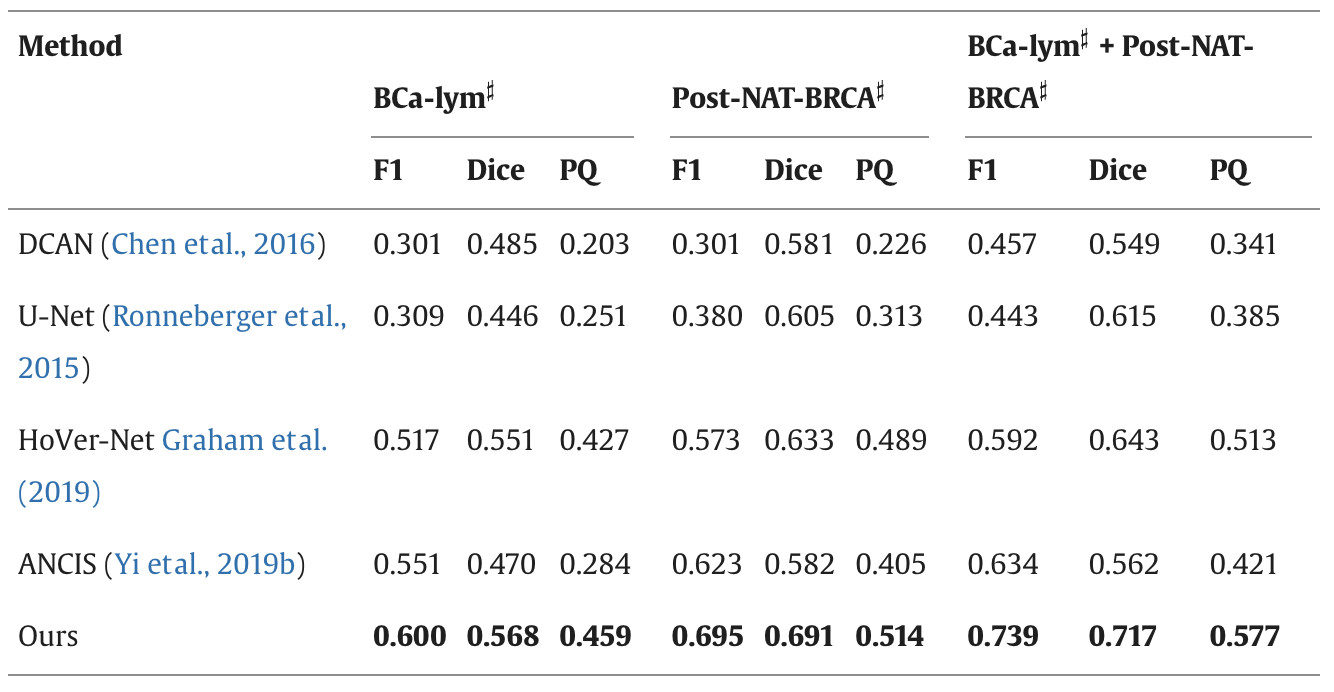
\includegraphics[width=14cm]{assets/images/rw-ddtn-generalize.png}
    \par\end{centering}
    \caption{Comparison of DDTN and baseline models in generalization}
    \label{fig:rw-ddtn-generalize}
\end{figure}

\section{Nuclei segmentation with point annotations from pathology images via self-supervised learning and co-training \cite{Lin2023}}
In the fourth work. The authors present a self-supervised approach that generates segmentation masks from point annotations of cell nuclei in H\&E stained images.

Two datasets were used and since each dataset was annotated using pixel-level annotations, these were converted to point annotations that were set approximately to the center of each mask. The datasets were:

\begin{itemize}
    \item MoNuSeg dataset, which we already mentioned earlier in this chapter. 24 images were used for training, 6 for validation, and 14 for testing.
    \item CPM dataset, containing 32 $500\!\times\!500$ or $600\!\times\!600$ H\&E stained images of four tumor types. 20 images were used for training, 4 for validation, and 8 for testing.
\end{itemize}

All the images for training were cropped to $250\!\times\!250$ patches with 125-pixel overlap for training - these are then randomly cropped further into $224\!\times\!224$ sub patches, rotated, flipped and zoomed. The images used for testing are cropped to $224\!\times\!224$ patches with 80-pixel overlap.

Their method contains three modules:

\begin{enumerate}
    \item Segmentation of nuclei with rough (not very precise) labels. Initial pixel-level masks are generated as follows: From point annotations using Voronoi diagram and \textit{k}-means clustering the Voronoi labels (a division of the image into convex polygons) and cluster labels (3 clusters in total - nuclei, background, ignored area) are generated. The H-component image is separated from the original H\&E stained image. Then the Residual U-Net network is trained using the Voronoi and cluster labels with cross-entropy loss to generate coarse pixel-level masks.
    \item Next in the co-training strategy, two segmentation networks are trained, where they supervise each other. The training data is split into two parts and each network is trained with one part. Apart from the two mentioned labels each of them also uses pseudo-labels generated by the other network which are stabilized using exponential moving average (EMA) where the averaged predicted labels are used to label the ignored area of the cluster label. The co-training loss is given by the Kullback-Lieber divergence.
    \item The self-supervised representation learning employs two U-Nets in sequential order, where the first U-Net computes the nuclei probability map (using the H-component images) and the second then reconstructs the colorized image from these maps.
\end{enumerate}

To integrate all of these modules, a final model is proposed. It has two networks, which are co-trained using Voronoi, cluster, and each other labels (with the EMA stabilization) and colorization loss. Each network consists of two U-Nets, the segmentation U-Net and the colorization U-Net. The ResNet-34 is used as a backbone network, pre-trained on the ImageNet dataset. The training hyperparameters were set as follows: initial learning rate of 0.001 reduced by a factor of 10 every 30 epochs, Adam optimizer, weight decay set to 0.0005. The colorizing network part is discarded during inference and only the segmentation part is used. The full architecture can be seen in figure \ref{fig:rw-self-sup-arch}.

\begin{figure}[H]
    \begin{centering}
    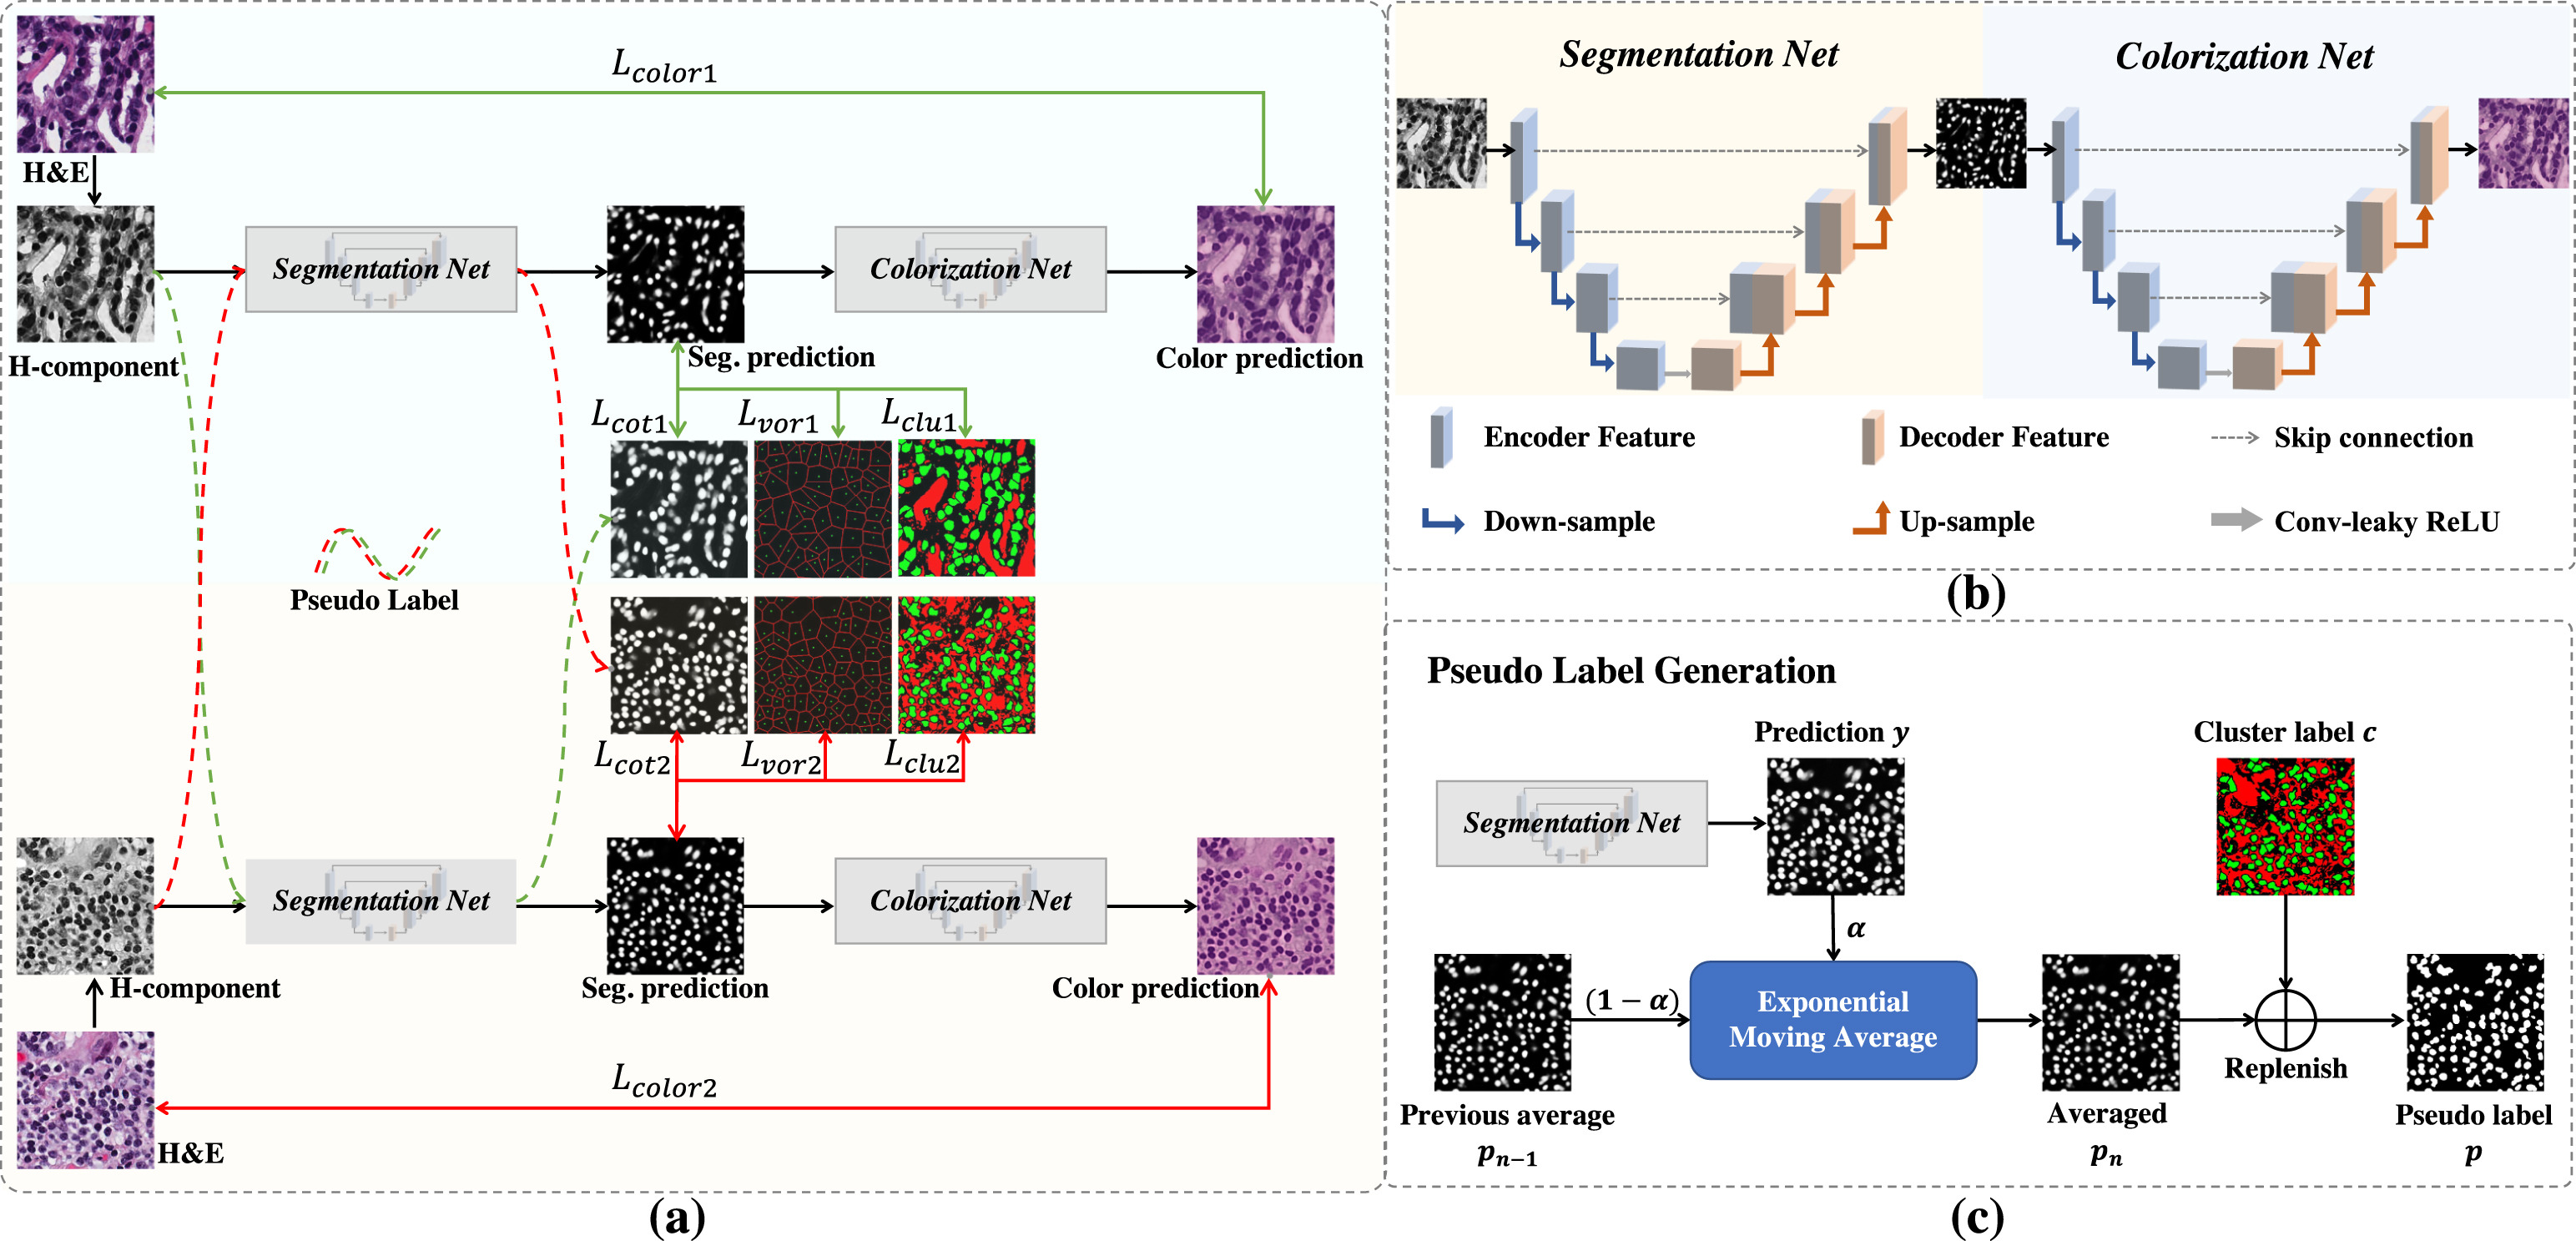
\includegraphics[width=14cm]{assets/images/rw-selfsup-arch.jpg}
    \par\end{centering}
    \caption{The architecture of proposed model}
    \label{fig:rw-self-sup-arch}
\end{figure}

Pixel accuracy, F1-score, Dice coefficient, Aggregated Jaccard Index, Detection Quality (DQ), Segmentation Quality (SQ), and Panoptic Quality (PQ) are used as the evaluation metrics. From the figure \ref{fig:rw-self-sup-results} we can see that the proposed network achieved better results on both datasets in almost all metrics when compared to other state-of-the-art models trained for weakly supervised nuclei segmentation with the same set of hyperparameters.

\begin{figure}[H]
    \begin{centering}
    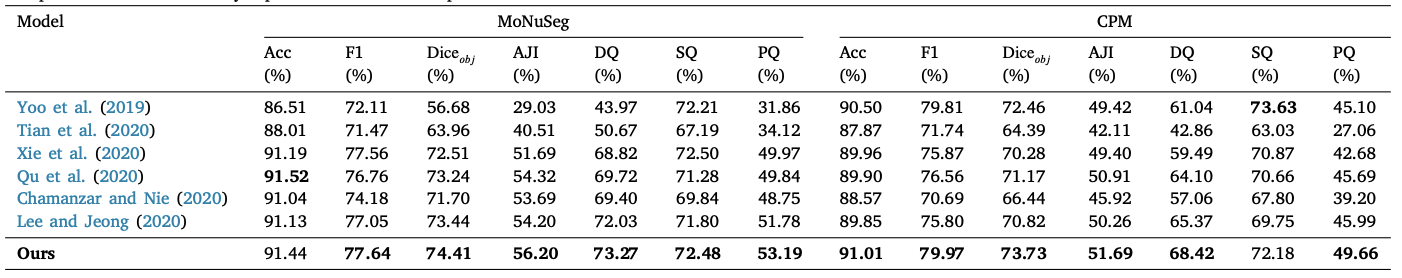
\includegraphics[width=14cm]{assets/images/rw-selfsup-results.png}
    \par\end{centering}
    \caption{The architecture of proposed model}
    \label{fig:rw-self-sup-results}
\end{figure}

\section{Weakly Supervised Deep Nuclei Segmentation With Sparsely Annotated Bounding Boxes for DNA Image Cytometry \cite{Liang2023}}
The last work focuses on segmenting cell nuclei in DNA image cytometry from bounding box annotations using a teacher-student network setup.

Two datasets were used:

\begin{itemize}
    \item DNA-ICM database, contains 23.485 images of cervical cancer screening stained with feulgen and eosin. Each image has $4096\!\times\!2816$ pixels. Together the dataset contains more than 1M cell nuclei. 18,266 images were selected for training and validation and 5,219 for testing. The authors used a semi-automated approach to get pixel-level masks for the test set. For the training and validation sets, they initially generated the pixel-level masks with traditional methods and then let experts refine them.
    \item ISBI14 dataset, containing 16 real and 945 synthetic images of cervical cytology. 8 real and 45 synthetic images were used for training, while the rest were used for testing.
\end{itemize}

Firstly, pseudo-masks are generated for each available bounding box by cropping out the box area and applying traditional segmentation methods, namely Otsu, K-means, and GrabCut. These initial pseudo-labels, along with the bounding boxes, are then used to train the teacher model. It produces pseudo-labels in the form of refined masks for ground truth nuclei labels (bounding boxes), and bounding boxes and masks for unlabelled nuclei. The student model then uses the ground truth labels and teacher-generated pseudo labels to further optimize the loss. The loss combining the supervised, weakly supervised, and unsupervised losses is used for the training of the student model.

Both the teacher and student models share the ResNet-50 with a feature pyramid network (with discarded level P6) as a backbone. The backbone is initialized with weights pre-trained on the ImageNet dataset. It is used to extract ROI features. Then both have the same architecture, the Mask R-CNN, which is, in total, trained for 32,000 iterations. The first 16,000 iterations are used to train the teacher model. Then the pseudo-labels generated by it are used for training the student model. The student model is initialized with the weights of the teacher model. The architecture can be seen in figure \ref{fig:rw-teacher-student}. The training hyperparameters were set as follows: weight decay of 0.0001; momentum of 0.9; initial learning rate of 0.01 and decreased by a factor of 10 after the 20,000th and 27,000th iterations.

\begin{figure}[H]
    \begin{centering}
    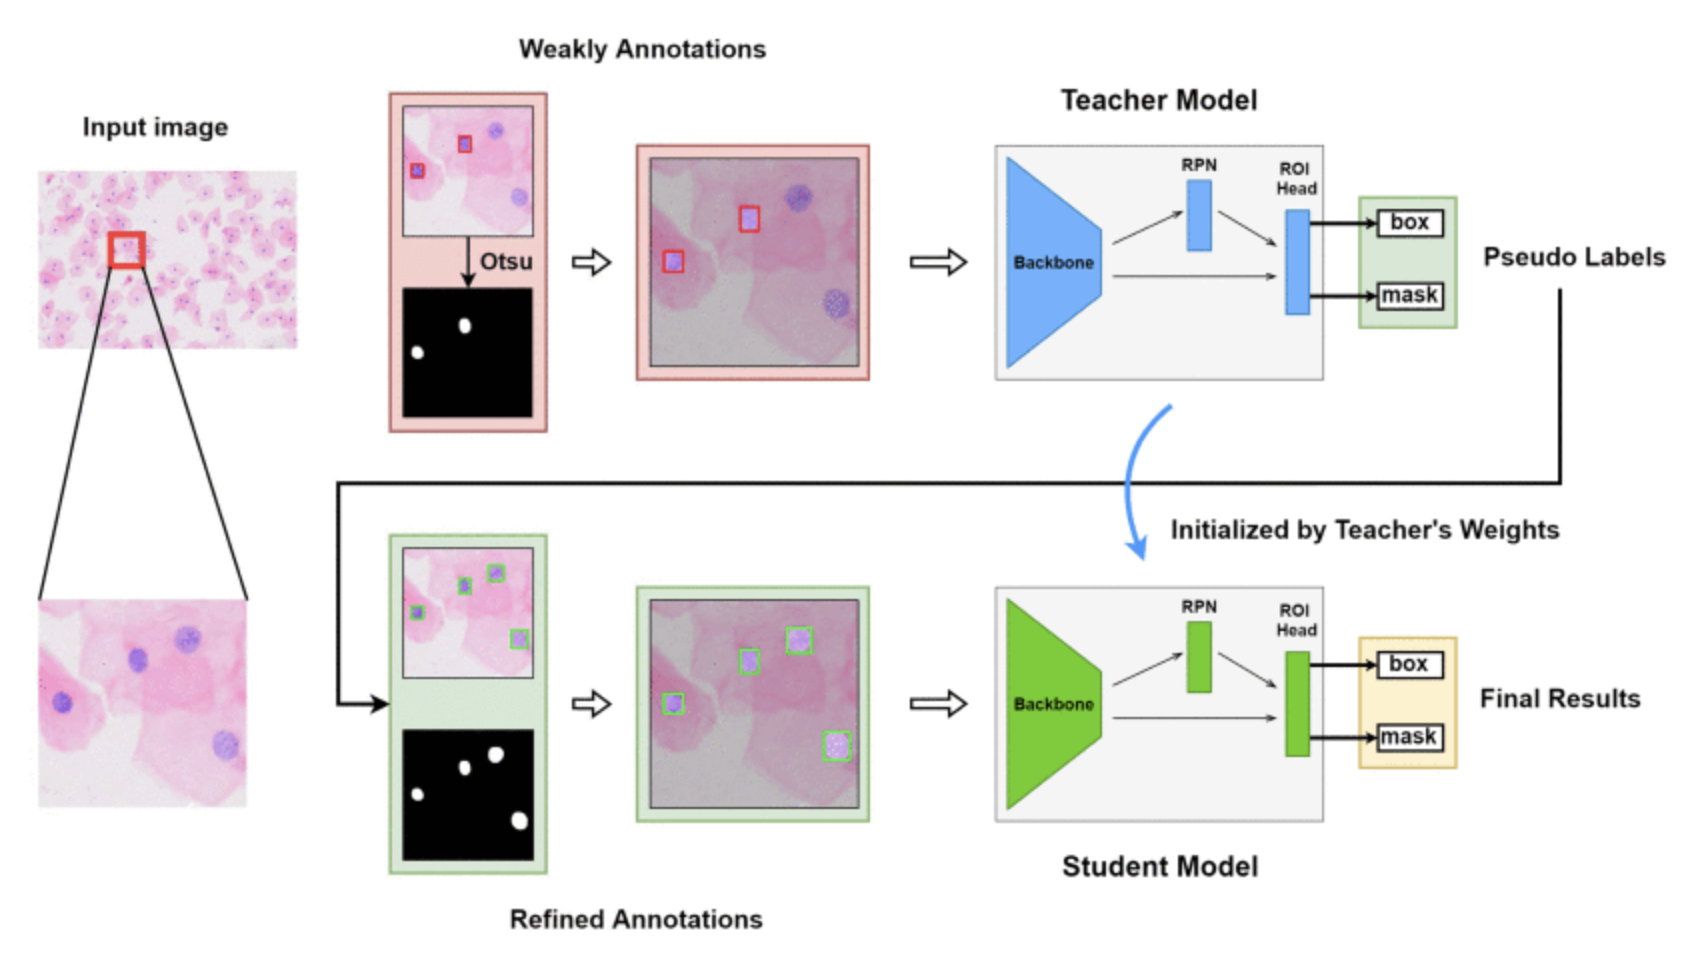
\includegraphics[width=14cm]{assets/images/rw-teacher-student.png}
    \par\end{centering}
    \caption{The architecture of the teacher-student model}
    \label{fig:rw-teacher-student}
\end{figure}

Precision, recall, pixel-level IoU, and Dice coefficient were used as evaluation metrics for nuclei segmentation. For cell detection, the average precision and recall over different IoU thresholds were used.

The comparison of results compared to other state-of-the-art weakly supervised methods can be seen in figures \ref{fig:rw-ts-seg} for segmentation and \ref{fig:rw-ts-det} for detection on the DNA-ICM dataset, where it achieved the best results compared to the other methods in all metrics but recall. Figure \ref{fig:rw-ts-seg-2} displays results comparison for segmentation on the ISBI14 dataset. Since this dataset is fully annotated with pixel-level masks, authors used these (either 100\% of them or 50\% of them) to generate the pseudo-labels. The model trained on this dataset was trained only for 100 epochs in total, 50 of them were the training of the teacher model. Again, their solution seemed superior in most of the metrics when compared to the other models.

\begin{figure}[H]
    \begin{centering}
    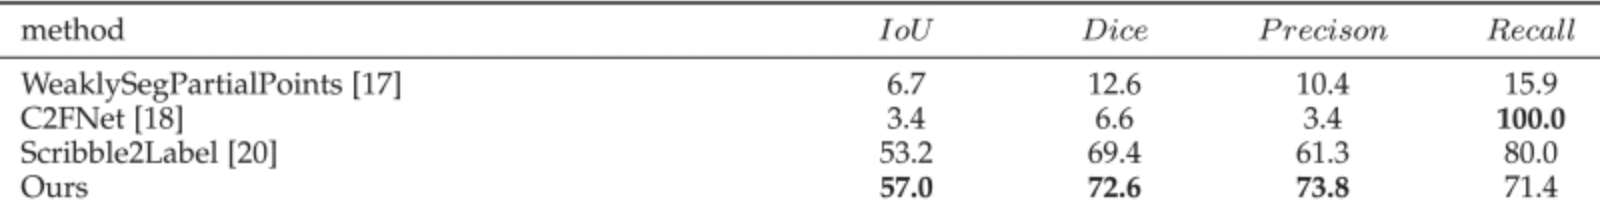
\includegraphics[width=14cm]{assets/images/rw-ts-seg.png}
    \par\end{centering}
    \caption{The comparison of results for segmentation on the DNA-ICM dataset}
    \label{fig:rw-ts-seg}
\end{figure}

\begin{figure}[H]
    \begin{centering}
    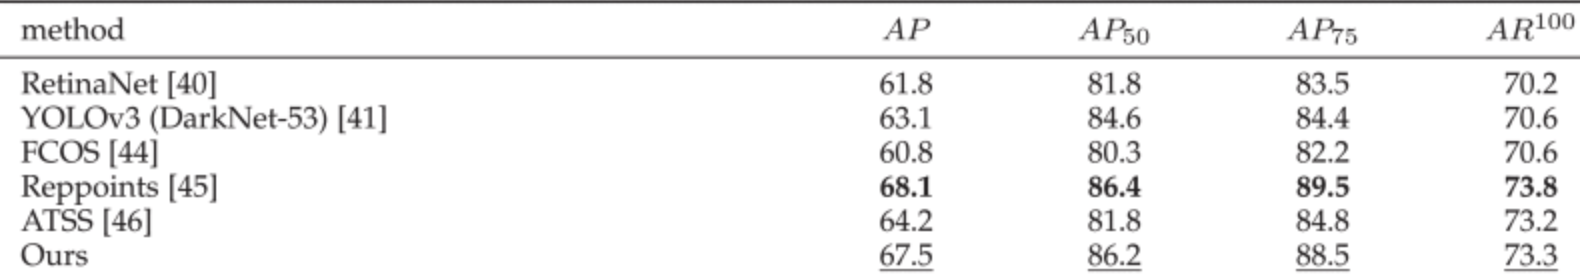
\includegraphics[width=14cm]{assets/images/rw-ts-det.png}
    \par\end{centering}
    \caption{The comparison of results for detection on the DNA-ICM dataset}
    \label{fig:rw-ts-det}
\end{figure}

\begin{figure}[H]
    \begin{centering}
    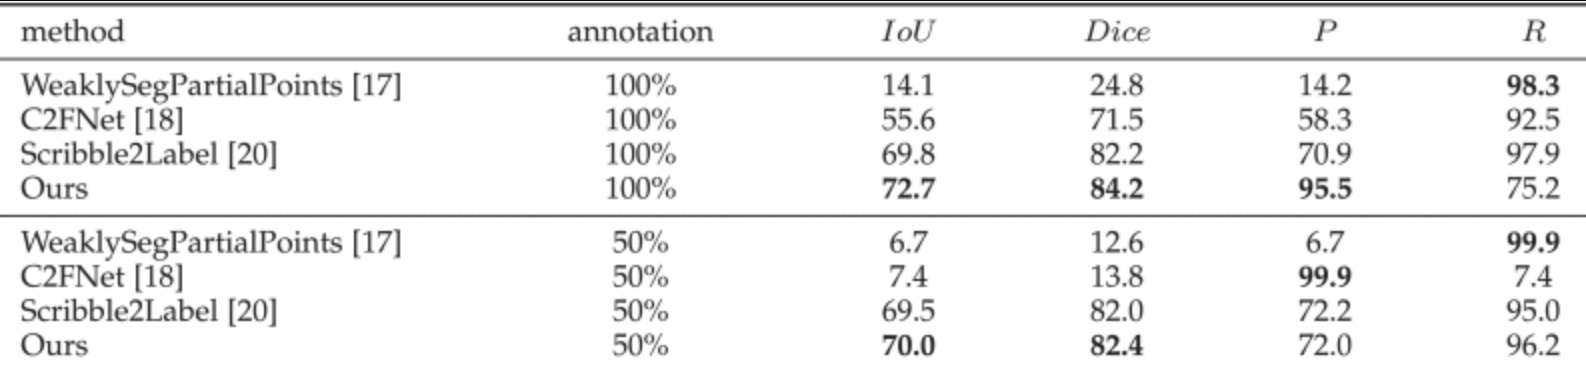
\includegraphics[width=14cm]{assets/images/rw-ts-seg-2.png}
    \par\end{centering}
    \caption{The comparison of results for segmentation on the ISBI14 dataset}
    \label{fig:rw-ts-seg-2}
\end{figure}

% Solution Concept
\clearpage\null
\chapter{Proposed Solution Concept}
\label{chap:solution-concept}

To successfully fulfil the defined objectives, we propose the solution described in this chapter. We will develop a robust framework capable of generating semantic segmentation masks for individual TILs from weak bounding box annotations. The high-level overview of architecture can be seen in figure \ref{fig:sc-main}. It can be split into three main parts (modules) each responsible for different tasks:

\begin{enumerate}
    \item \textbf{Image preprocessing module} will contain various image preprocessing techniques, such as normalization of images.
    \item \textbf{Pseudo-label generating module} will be responsible for generating pseudo-labels in the form of segmentation masks.
    \item \textbf{Deep learning model} will use the preprocessed images and the generated pseudo-masks to make predictions.
\end{enumerate}

\begin{figure}[H]
    \begin{centering}
    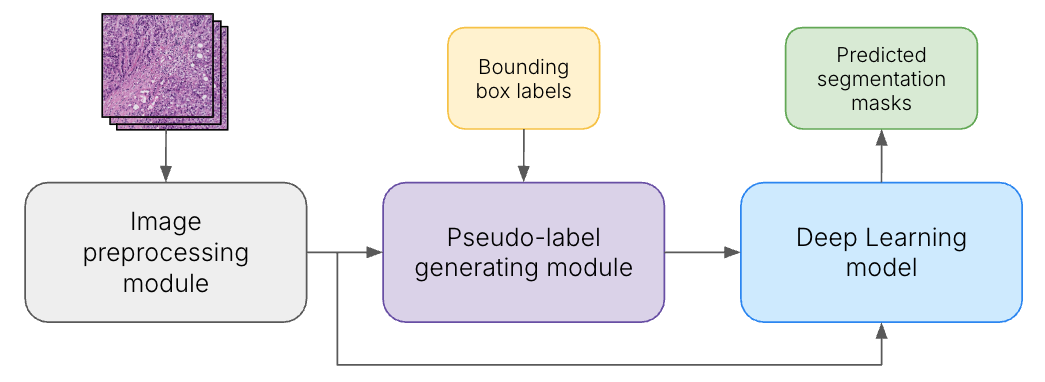
\includegraphics[width=14cm]{assets/images/sc-main.png}
    \par\end{centering}
    \caption{The high-level overview of the proposed architecture}
    \label{fig:sc-main}
\end{figure}

We describe each module in more detail in the following sections.

\section{Image Preprocessing Module}
This module will perform global preprocessing of images. Since the WSIs come from different institutes, and different surgical procedures, the normalization is a necessary step. We already performed first experiments using Macenko normalization, and we mention these in the chapter \ref{chap:prelim-exp}.

The randomly selected image as a reference image for Macenko normalization laid suboptimal results.We have considered other approaches to select a reference image, but as recent study \cite{Ivanov2024} showed, that when selecting only a single reference image for Macenko normalization, the results will always be biased and suboptimal. Therefore we would like to try experimenting with their proposed method of selecting multiple images to obtain better results. We would also like to try the normalization method used in \cite{Vahadane2015}, which showed promising results.

\section{Pseudo-label Generating Module}
The main task of this module will be generation of pseudo-labels in the form of pixel-level masks. For this purpose we crop out the individual cells with respect to their bounding box ground truth labels. Then we want to apply different traditional segmentation methods, such as GrabCut, watershed, and Otsu to obtain the mask for a single cell. We would also like to test tools such as QuPath and Cell Profiler.These individual masks will be then combined back into the large mask for the original large image. This large pseudo-masks will then be used by the deep learning model during training. The performance of these methods can be increased with different preprocessing techniques such as CLAHE or power law (gamma) transformation. This means that this module will also be responsible for some local image processing. We already performed preliminary experiments on this topic, which we write about in chapter \ref{chap:prelim-exp}.

\section{Deep Learning Model}
The final module will consist of a deep learning model. We would like to perform experiments with different architectures of CNN-based networks, and possibly Vision Transformers as well. We did not yet finalized the set of models we would like to experiment with but based on the related work, we consider U-Net-based architectures, namely Residual U-Net and Attention U-Net. The evaluation metrics such as IoU and Dice score will be used for final evaluation and the best model will be selected and fine-tuned.



% Preliminary Experiments
\clearpage\null
\chapter{Preliminary Experiments}


% ----- IN FINAL WORK -----
% Conclusion
%\clearpage\null
%\chapter{Conclusion}



% Resume
%\clearpage\null
%\chapter*{Resumé}

% -------------------------

% Bibliography
\clearpage\null

\printbibliography[heading=references,segment=\therefsegment,resetnumbers=true]

\end{refsegment}

% ----- IN FINAL WORK -----
% Appendix
% \appendix

% \clearpage\null
% \chapter{Plan of Work \label{appendix:plan} }
\renewcommand{\thepage}{A-\arabic{page}}
\setcounter{page}{1}

\textbf{Bachelor's thesis evidence number:} FIIT-100241-116291

\section{Winter Semester}
In Table \ref{tab:winter_plan}, we can see a summarized plan of work for the winter semester. During this time, we familiarizing ourselves with the whole topic of weak segmentation and traditional methods of computer vision. We also explored the available datasets, and after we selected the TIGER dataset, we explored it in more depth. We were studying the state-of-the-art, gathering information, and running preliminary experiments. Later, we constructed an initial concept of experiments that should be performed. The experiments were performed more slowly than we anticipated because of the complicated dataset features, which caused us a slight delay, but on the other hand, we were now very confident with the dataset usage and knew better what we should do next to be successful.

\begin{table}[h!]
\centering
\begin{tabular}{|c|p{12.5cm}|}
\hline
\textbf{Week} & \textbf{Planned Work} \\ 
\hline
\hline
1-2 & Literature review on digital pathology and TIL detection. \\ 
\hline
3-6 & Study of deep learning techniques and architectures (CNNs, U-Net, Vision Transformers) and different pseudo-label generation techniques (GrabCut, watershed, Otsu). \\
\hline
7 & Familiarization with the TIGER dataset. \\
\hline
8-10 & Initial development of the pipeline to convert bounding box annotations to pixel masks. Preparing the mid-term report. \\ 
\hline
11-13 & Preparing mid-term report, finishing analysis, summarizing progress and findings. \\ 
\hline
\end{tabular}
\caption{Plan of Work for Winter Semester}
\label{tab:winter_plan}
\end{table}

\section{Summer Semester}
The Table \ref{tab:summer_plan} displays the plan for the summer semester. During this time, we had a large portion of work to do. We selected a TNBC dataset, which was fully annotated, as another dataset to be included in this work. We had to implement 24 different strategies for pseudo-mask generation and then perform the model training on all of them, and select the best one. We also came up with different methods of generating pseudo-masks (fusing the original 24 pseudo-masks), meaning that we had another large portion of experiments to perform. Then, a transfer learning approach idea came for the final model, which was the most successful. During the whole semester, we performed almost 600 trainings, and in comparison to the winter semester, the whole work has picked up speed. As we mentioned, we were adding more experiments as the work progressed. We were able to successfully build the pipeline of computer vision operations that generated different pseudo-masks, prepare the U-Net segmentation model, and were able to train it in the Azure cloud environment. 

Given the many challenges we had to overcome, like the weakly annotated TIGER dataset, a very small TNBC dataset, inconsistencies across the datasets, and the challenging task of segmenting only a specific class of cell nuclei (not all cell nuclei), we conclude that this plan was fully adhered to and completed.

\begin{table}[h!]
\centering
\begin{tabular}{|c|p{12.5cm}|}
\hline
\textbf{Week} & \textbf{Planned Work} \\ 
\hline
\hline
1-2 & Continuing with the computer vision pipeline development. \\
\hline
3 & Testing and refining the pseudo-label generation algorithm. \\ 
\hline
4-8 & Implementing, training, and evaluation of the U-Net segmentation model trained with various pseudo-masks. Analysis of the model using evaluation metrics (IoU, Dice coefficient). \\ 
\hline
9 & Final experiments, preparation of the final thesis outline. \\ 
\hline
10-12 & Writing and presenting the final report with results and conclusions. \\ 
\hline
13 & Submission of final thesis. \\ 
\hline
\end{tabular}
\caption{Plan of Work for Summer Semester}
\label{tab:summer_plan}
\end{table}

\chapter{Technical Documentation \label{appendix:td} }
\renewcommand{\thepage}{B-\arabic{page}}
\setcounter{page}{1}

\section{Project's folder structure}
\label{projects-folder-structure}

\verbatiminput{assets/folder-tree.txt}

\section{Description of folders and
files}\label{description-of-folders-and-files}

\subsection{\texttt{root} directory}\label{root-directory-files}

\paragraph{.amlignore}
Here is a list of folders and files that are ignored when a job is
submitted to the Azure ML platform. When a job is submitted, Azure takes
a snapshot of the directory it is given as the source directory. The
files listed in \texttt{.amlignore} will be ignored by this operation.

\paragraph{.gitignore}
Files to be ignored by the Git versioning system.

\paragraph{main.ipynb}
In this Jupyter notebook, the whole preprocessing, pseudo-mask generating, and pseudo-mask fusing pipeline can be run. It also provides
the visualizations of preprocessed images and pseudo-masks. This notebook has already been executed, so you can also see the outputs of each cell. Open
the \texttt{main.ipynb }to see it.

\paragraph{main.py}
This is the main training and evaluation script. It can be run both
locally and on the Azure ML platform. See Section \ref{how-to-run-the-demo} to see both possible
options.

\paragraph{README.md}
In this file, the document with the same content as in this Chapter is.

\paragraph{requirements.txt}
Contains Python dependencies that need to be installed to run the project.

\subsection{\texttt{config} directory files}
\label{config-directory-files}

\paragraph{azure\_connect\_example.json}
Contains the information required to authenticate and connect to your
Azure ML Workspace. You will need to fill out this configuration file, otherwise, the
connection will not be successful. Keep the structure, just change the
values to match your account.

\paragraph{azure\_job.yaml}
Contains all configuration values that are used to submit the job run,
which will train the model. These include the data asset information,
the environment information (environment where the job will run), the
job information (like source directory to push to Azure ML, compute
target, etc.), and the arguments to be passed to the \texttt{main.py}
function once it is executed.

\paragraph{azure\_upload\_data.yaml}
Here is the information about the folder you want to upload to the
Azure storage, the destination folder on Azure ML, and options to
overwrite already existing files and see the progress of the whole
process.

\paragraph{model\_train\_base.yaml}
Contains the hyperparameters that are used by the model during the
training and evaluation. It also contains the option to load the
pre-trained model.

\paragraph{paths.yaml}
This file contains all paths, or parts of paths, where the images are
being stored, created, modified, and updated, and from which are loaded
during the preprocessing. The whole folder structure for the
preprocessing and pseudo-mask creation is created in the
\texttt{./main.ipynb} notebook, where the full paths are built. Note that by default, all file manipulations are performed under
the \texttt{/example\_data/} directory (unless changed in this config).
For the demo, we recommend keeping this
configuration file as is. For the real preprocessing, we advise changing the
\texttt{root\_data\_dir} value to point to the \texttt{/data} directory.

\subsection{\texttt{data} and \texttt{example\_data} directories}\label{data-and-example_data-directories}

The \texttt{data} directory contains four main subdirectories. Here the
images and annotations of the respective datasets reside
(TIGER\footnote{\url{https://tiger.grand-challenge.org/Data/}} and TNBC\footnote{\url{https://zenodo.org/records/3552674}} datasets). The
\texttt{/data/raw\_*} folders contain the raw images and annotations
(bounding box for TIGER - in the COCO JSON format\footnote{\url{https://roboflow.com/formats/coco-json}}, PNG
masks for TNBC). The \texttt{/data/preprocessed\_*} directories contain
more subdirectories that are created during the run of the
\texttt{./main.ipynb} notebook. The most important ones are:

\begin{itemize}
\item
  \texttt{/data/preprocessed\_*/patches/images} which contains the
  $128\!\times\!128$ normalized image patches
\item
  \texttt{/data/preprocessed\_*/patches/masks} which contains the
  $128\!\times\!128$ mask (or pseudo-mask) patches
\item
  \texttt{/data/preprocessed\_tnbc/patches/folds} which contains TNBC
  image and mask patches, but split into folds, where each fold directory
  has \texttt{/data/preprocessed\_tnbc/patches/folds/fold\_*/images} and
  \texttt{/data/preprocessed\_tnbc/patches/folds/fold\_*/masks} folder
\end{itemize}

Note that this directory is meant to be used for real preprocessing, and
you need to put here the correct images and annotations yourself.

The \texttt{/example\_data} directory follows the exact same structure,
but already contains 10 example images from the TIGER dataset in the
\texttt{/data/raw\_tiger/images} subdirectory, the
\texttt{tiger-coco.json} file with the TIGER bounding box annotations in
the \texttt{/data/raw\_tiger} subdirectory, and 4 images from the TNBC
dataset in the \texttt{/data/raw\_tnbc/images} subdirectory and their
corresponding masks in the \texttt{/data/raw\_tnbc/masks} subdirectory.
This directory is by default listed as the \texttt{root\_data\_dir} in
the \texttt{/configs/path.yaml} file, so in order to run the
\hyperref[how-to-run-the-demo]{Demo} you do not need to change anything
in the \texttt{/configs/path.yaml} file.

\subsection{\texttt{models} directory}\label{models-directory}

Here, the models that you wish to save and use for future fine-tuning or
reference should be placed. We do not include any pre-trained model here,
since the \texttt{.ckpt} files are around 300MB in size.

\subsection{\texttt{src/azure} directory}\label{srcazure-directory}

\paragraph{azure\_conda.yaml}
Defines the dependencies that will be installed within Azure ML
environment.

\paragraph{azure\_train.ipynb}
From this Jupyter notebook, the training is managed. This involves
authenticating, pulling the correct data asset path, creating the
environment, and submitting the job to Azure ML. Use the
\texttt{/configs/azure\_connect\_example.json},
\texttt{/configs/azure\_job.yaml} and
\texttt{/configs/model\_train\_base.yaml} to manage the configuration of
parameters.

\paragraph{azure\_upload\_data.ipynb}
This Jupyter notebook is used to upload a locally stored folder to the
remote Azure ML data storage. Use the
\texttt{/configs/azure\_upload\_data.yaml} to manage the configuration
of parameters.

\subsection{\texttt{src/models} directory}\label{srcmodels-directory}

\paragraph{inference.ipynb}
In this Jupyter notebook, you run the inference of the model. A
pretrained model is required for this stage. The predictions are
visualized. The inference is run on the
\texttt{tnbc\_sample\_img\_patch} image from the
\texttt{/configs/paths.yaml} configuration file.

\paragraph{model\_factory.py}
Here we define the architecture of the model.

\paragraph{til\_dataset.py}
This file defines a utility class that is used to output the image and
mask pairs that are further used during the training and evaluation by
the PyTorch \texttt{DataLoader}s.

\subsection{\texttt{src/*.py} files}\label{src.py-files}

\paragraph{image\_preprocessor.py}
Contains the \texttt{ImageProcessor} class that groups all the
preprocessing functionalities.

\paragraph{image\_stats.py}
Contains the \texttt{ImageStats} class that prints the statistics of the
folder that contains images, like average image height, width, area,
etc.

\paragraph{mask\_generator.py}
Contains the \texttt{MaskGenerator} class that groups all the
mask-generating and mask-fusing functionalities.

\paragraph{sample.py}
Contains the \texttt{Sample} class that is used for visualization of the
image and its mask.

\paragraph{utils.py}
Contains all other utility functionalities, for example, for opening and
loading \texttt{.json} and \texttt{.yaml} files.

\section{Installation guide}\label{installation-guide}

\subsection{Prerequisites}\label{prerequisites}

Below, we list the necessary software requirements: 

\begin{itemize}
    \item Python version 3.12+
    \item \texttt{pip} version 23.2+
    \item Internet access to download packages
    \item Weights and Biases account for model logging
    \item Azure ML
access (if you wish to train models there)
\end{itemize}

\subsection{Clone the repository}\label{clone-the-repository}

Clone this repository and navigate into it:

\begin{bashlisting}
git clone <repository-name>
cd <cloned-repository-name>
\end{bashlisting}

Alternatively, you can download the \texttt{.zip} file of this project,
unpack it, and open a terminal within it.

\subsection{Set up the Python
environment}\label{set-up-the-python-environment}

Set up the virtual environment using \texttt{pip} (or create Conda
environment, but we will be using \texttt{pip}).

Using MacOS:

\begin{bashlisting}
python3 -m venv .venv
source .venv/bin/activate
\end{bashlisting}

or Windows (from PowerShell):

\begin{pslisting}
python -m venv .venv
.\.venv\Scripts\Activate.ps1 
\end{pslisting}

\subsection{Install dependencies}\label{install-dependencies}

Dependencies are listed in the \texttt{requirements.txt} file. To
install them all, use:

\begin{bashlisting}
pip install -r requirements.txt
\end{bashlisting}

\section{How to run the Demo}
\label{how-to-run-the-demo}

Here we present a way to run the demo version (using the demo data
placed in the \texttt{/example\_data} folder). Be aware of the fact,
that since we only have 10 training images and 4 testing images in this
demo, the model performance will be poor. This is just to showcase how
the project works. Also, note that our project works with the PNG images only.

\subsection{Preprocessing and pseudo-mask
creation}\label{preprocessing-and-pseudo-mask-creation}

\begin{enumerate}
\item
  Navigate to the \texttt{./main.ipynb} Jupyter notebook.
  You will notice that the notebook is already run (for the
  demonstration). Feel free to examine it before trying to run anything.
\item
  Next, make sure that you clear all outputs (to avoid any confusion)
  and start running it cell after cell (or all at once). You will notice
  that under the \texttt{/example\_data/processed\_*} directories,
  different subdirectories will appear. Those will be populated with
  different images or versions of images and masks during the
  preprocessing and pseudo-mask creation. During the execution of the
  cells, you will also see the textual and visual output responses.
\item
  After the whole notebook is executed, feel free to examine the different
  subdirectories that were created - but be careful not to delete, move,
  or rename any of them or their contents.
\item
  The data is now prepared for the training.
\end{enumerate}

\subsection{Training on Azure}\label{a-training-on-azure}

Here we describe the necessary steps that are required to be
able to train the model on the Azure ML platform.

\begin{enumerate}
\item Ensure you have access to an Azure ML workspace and all the required
  information. Fill them in the
  \texttt{/configs/azure\_connect\_example.json} configuration file.
\item Ensure that the information in the
  \texttt{/configs/azure\_upload\_data.yaml} configuration file is
  correct. You will need to input the correct
  \texttt{target\_path} as this is not provided by us!
\item Then navigate into the \texttt{./src/azure/azure\_upload\_data.ipynb}
  and run it cell by cell. Be especially careful with the local and
  remote directory paths. The contents of the local directory will be
  copied into the remote directory.
\item After the data has been uploaded, you will need to create the Azure
  Data Asset. See the official Azure documentation\footnote{\url{https://learn.microsoft.com/en-us/azure/machine-learning/how-to-create-data-assets}} how to do it.
\item Then you will need to create an Azure compute instance. See this official Azure documentation\footnote{\url{https://learn.microsoft.com/en-us/azure/machine-learning/how-to-create-compute-instance}} for precise instructions.
\item Next, you will need to modify \texttt{/configs/azure\_job.yaml} file,
  as we cannot provide defaults for certain variables:
  \begin{itemize}
  \item
    See the \texttt{dataset} top-level key. You need to input the
    \texttt{name} of the Data Asset and its \texttt{version} you created
    in Step 4.
  \item
    See the \texttt{job} top-level key. You need to change the
    \texttt{job.compute} to have the name of the compute instance target
    you created in Step 5.
  \item
    See the \texttt{jobs.args.wandb} key. You will need to input your
    Weights and Biases key, so the training and evaluation process can
    be monitored. See the official guide\footnote{\url{https://docs.wandb.ai/support/find_api_key/}} on how to get the key.
  \end{itemize}
\item
  \emph{(Optional)} If you wish, you can try to change the model
  parameters; you can do so in the
  \texttt{/configs/model\_train\_base.yaml} file, but this step is
  optional.
\item
  Now navigate to the
  \texttt{./src/azure/azure\_train.ipynb} and follow
  the instructions within it to submit the training and evaluation job
  to the Azure ML platform.
\item
  During the training, you can see and monitor the whole process in your
  Weights and Biases account.
\item
  After the training and evaluation are done, look for the
  \texttt{outputs} folder in the job details on the Azure ML platform.
  It should be in the \emph{Outputs + logs} tab, but the Azure ML
  platform UI changes constantly.
\item
  You can download the trained model from the
  \texttt{outputs/checkpoints/best.ckpt}. Be aware that the checkpoint
  file is around 300MB in size.
\end{enumerate}

\subsection{Training locally}\label{b-training-locally}

This option presents a way to run the training and evaluation
locally. Note that the Demo will work just fine, since there is only a
fraction of the size of a real dataset, but when training with a large
dataset, the time to train the model locally can be significantly
longer.

Follow these steps:

\begin{enumerate}
    \item \emph{(Optional)} If you wish, you can try to change the model parameters in the \texttt{/configs/model\_train\_base.yaml} file, but this step is optional.
    \item Run the \texttt{main.py} script. Be sure to input your correct Weights and Biases key. See the official guide\footnote{\url{https://docs.wandb.ai/support/find_api_key/}} on how to get the key.
    \begin{bashlisting}
python3 main.py \
  --data_path './example_data' \
  --wandb '<your-wandb-key>' \
  --train_images_path 'processed_tiger/patches/images' \
  --train_masks_path 'processed_tiger/patches/masks/fused_leave_1_out' \
  --test_images_path 'processed_tnbc/patches/images' \
  --test_masks_path 'processed_tnbc/patches/masks'
\end{bashlisting}
    
    \item During the training, you can see and monitor the whole process in your Weights and Biases account.
    \item Once the training finished, you will notice that a new \texttt{/outputs} directory was created. This contains both the trained model in the \texttt{/outputs/checkpoints/best.ckpt} file and the raw Weights and Biases logs in the \texttt{outputs/wandb} folder. Furthermore, it contains a \texttt{outputs/test\_results.json} with the evaluation metrics from the evaluation phase.
\end{enumerate}

\subsection{Inference}\label{inference}

To see how the model works during inference, navigate
to the \texttt{./src/models/inference.ipynb}. Notice
that this notebook has already been executed as well; feel free to examine it and then
clear the outputs (to avoid any confusion). You will need to
input the path to the trained model \texttt{.ckpt} file, as we do
not provide a trained model in the demo. Run the notebook and
see the results!

% \clearpage\null
% \chapter{Contents of Included CD–ROM \label{cha:cdrom} }

CD–ROM included to the thesis contains following files:

\begin{itemize}
\item \texttt{/file1} --- First file
\item \texttt{/file2} --- Second file
\end{itemize}

% -------------------------

\end{document}
